
% VLDB template version of 2020-08-03 enhances the ACM template, version 1.7.0:
% https://www.acm.org/publications/proceedings-template
% The ACM Latex guide provides further information about the ACM template

\documentclass[sigconf, nonacm]{acmart}

\usepackage{dsfont}          % <-- add this
% \newcommand{\ind}{\mathds{1}}% optional shorthand
\usepackage{enumitem}
\usepackage{bbold}            % 
\newcommand{\ind}{\mathbb{1}} % shorthand (uses bbold)

\usepackage{algorithm}      % wraps the figure, gives caption & numbering
%            ––or––
\usepackage{algorithmicx}    % plain syntax (e.g. \STATE, \FOR … \ENDFOR)

\usepackage{algpseudocode}  % nicer pseudocode keywords (from the same author)
\usepackage{booktabs,subcaption}
\usepackage{multirow}
\usepackage{multicol}
\usepackage{booktabs}
\usepackage{siunitx}
\usepackage{array}
% \renewcommand{\tabularxcolumn}[1]{m{#1}}
\usepackage{svg}
\usepackage{arydshln}
\usepackage[htt]{hyphenat}

\usepackage{booktabs}
\usepackage{enumitem}
\usepackage{listings}

\usepackage{booktabs,tabularx,array,enumitem}
\newcolumntype{L}[1]{>{\raggedright\arraybackslash}p{#1}}
\newcolumntype{Y}{>{\raggedright\arraybackslash}X}

\lstdefinelanguage{SQL}{
  keywords={SELECT, FROM, WHERE, GROUP, BY, UPDATE, SET, INSERT, INTO, VALUES, AVG, SUM, COUNT},
  keywordstyle=\bfseries,
  basicstyle=\ttfamily\small,
  sensitive=false
}

\sisetup{
  detect-all,
  round-mode         = places,
  round-precision    = 4,
  table-format       = 3.4,
  detect-weight      = true,          % <—  key line
  detect-inline-weight = math         % <—  key line
}

\newcommand{\best}[1]{{\bfseries #1}} % now safe inside S columns
\makeatletter
\algrenewcommand\alglinenumber[1]{\footnotesize\arabic{ALG@line}:}
\makeatother

\usepackage{tabularx}   % flexible-width columns (X) and \arraybackslash
\usepackage{bbm}
\usepackage{amsmath}
\usepackage{graphicx}
\usepackage{enumitem}
%% The following content must be adapted for the final version
% paper-specific
\newcommand\vldbdoi{XX.XX/XXX.XX}
\newcommand\vldbpages{XXX-XXX}
% issue-specific
\newcommand\vldbvolume{14}
\newcommand\vldbissue{1}
\newcommand\vldbyear{2020}
% should be fine as it is
\newcommand\vldbauthors{\authors}
\newcommand\vldbtitle{\shorttitle} 
% leave empty if no availability url should be set
\newcommand\vldbavailabilityurl{URL_TO_YOUR_ARTIFACTS}
% whether page numbers should be shown or not, use 'plain' for review versions, 'empty' for camera ready
\newcommand\vldbpagestyle{plain} 

\newcommand{\lrow}[1][]{\ell_{#1\mathrm{row}}}   % 例: \lrow        →  \ell_{,\mathrm{row}}
\newcommand{\lcol}[1][]{\ell_{#1\mathrm{col}}}   % 例: \lcol[t]     →  \ell_{t,\mathrm{col}}
\newcommand{\lengine}[2]{\ell_{#1\mathrm{#2}}}   % 通用: \lengine{i}{row}

\newcommand{\zxh}[1]{\textcolor{blue}{#1}}

\usepackage{siunitx}
\usepackage[normalem]{ulem} %

\sisetup{
  detect-weight         = true ,
  detect-inline-weight  = math ,
  round-mode            = places ,
  round-precision       = 4
}

\usepackage{xspace}
\newcommand{\dispatcher}{AQD\xspace}


\begin{document}
\title{\dispatcher: Online Adaptive Query Dispatcher for HTAP Databases}

% online adaptive dispatch strategy.


% Scene-Aware Row/Column Dispatch for HTAP Databases via Mixture-of-Experts Boosting 

% 从特殊且重要的场景入手,做选择对整体的查询影响很大。白天TP,晚上AP。故事更圆满,结果更好。他自己想不到,但是说出来他感兴趣的点。别人要对这个问题感兴趣。TP多的场景,AP多的场景。

%%
%% The "author" command and its associated commands are used to define the authors and their affiliations.
\author{Yang Wu}
\affiliation{%
  \institution{Department of Computer Science, Tsinghua University}
  \streetaddress{No. 30, Road Shuangqing, Haidian District}
  \city{Beijing}
  \state{China}
  \postcode{100084}
}
\email{wu-y22@mails.tsinghua.edu.cn}

\author{Tongliang Li}
\affiliation{%
  \institution{Alibaba Group}
  \streetaddress{No. 1008, Streat Dengcai, Sandun Town, Xihu District}
  \city{Hangzhou}
  \state{China}
  \postcode{310013}
}
\email{litongliang.ltl@alibaba-inc.com}

\author{Xuanhe Zhou}
\affiliation{%
  \institution{Department of Computer Science, Shanghai Jiao Tong University}
  \streetaddress{No. 800, Road Dongchuan, Minhang District}
  \city{Shanghai}
  \state{China}
  \postcode{200240}
}
\email{zhouxh@cs.sjtu.edu.cn}

\author{Jianying Wang}
\affiliation{%
  \institution{Alibaba Group}
  \streetaddress{No. 1008, Streat Dengcai, Sandun Town, Xihu District}
  \city{Hangzhou}
  \state{China}
  \postcode{310013}
}
\email{beilou.wjy@alibaba-inc.com}

\author{Xinjun Yang}
\affiliation{%
  \institution{Alibaba Group}
  \streetaddress{No. 1008, Streat Dengcai, Sandun Town, Xihu District}
  \city{Hangzhou}
  \state{China}
  \postcode{310013}
}
\email{xinjun.y@alibaba-inc.com}

% \author{Feifei Li}
% \affiliation{%
%   \institution{Alibaba Group}
%   \streetaddress{No. 1008, Streat Dengcai, Sandun Town, Xihu District}
%   \city{Hangzhou}
%   \state{China}
%   \postcode{310013}
% }
% \email{lifeifei@alibaba-inc.com}

\author{Wenchao Zhou}
\affiliation{%
  \institution{Alibaba Group}
  \streetaddress{No. 1008, Streat Dengcai, Sandun Town, Xihu District}
  \city{Hangzhou}
  \state{China}
  \postcode{310013}
}
\email{zwc231487@alibaba-inc.com}


\author{Chunxiao Xing}
\affiliation{%
  \institution{Beijing National Research Center for Information Science and Technology, Tsinghua University}
  \streetaddress{No. 30, Road Shuangqing, Haidian District}
  \city{Beijing}
  \state{China}
  \postcode{100084}
}
\email{xingcx@tsinghua.edu.cn}

\author{Yong Zhang}
\affiliation{%
  \institution{Beijing National Research Center for Information Science and Technology, Tsinghua University}
  \streetaddress{No. 30, Road Shuangqing, Haidian District}
  \city{Beijing}
  \state{China}
  \postcode{100084}
}
\email{zhangyong05@tsinghua.edu.cn}

% \author{Lars Th{\o}rv{\"a}ld}
% \orcid{0000-0002-1825-0097}
% \affiliation{%
%   \institution{The Th{\o}rv{\"a}ld Group}
%   \streetaddress{1 Th{\o}rv{\"a}ld Circle}
%   \city{Hekla}
%   \country{Iceland}
% }
% \email{larst@affiliation.org}

% \author{Valerie B\'eranger}
% \orcid{0000-0001-5109-3700}
% \affiliation{%
%   \institution{Inria Paris-Rocquencourt}
%   \city{Rocquencourt}
%   \country{France}
% }
% \email{vb@rocquencourt.com}

% \author{J\"org von \"Arbach}
% \affiliation{%
%   \institution{University of T\"ubingen}
%   \city{T\"ubingen}
%   \country{Germany}
% }
% \email{jaerbach@uni-tuebingen.edu}
% \email{myprivate@email.com}
% \email{second@affiliation.mail}

% \author{Wang Xiu Ying}
% \author{Zhe Zuo}
% \affiliation{%
%   \institution{East China Normal University}
%   \city{Shanghai}
%   \country{China}
% }
% \email{firstname.lastname@ecnu.edu.cn}

% \author{Donald Fauntleroy Duck}
% \affiliation{%
%   \institution{Scientific Writing Academy}
%   \city{Duckburg}
%   \country{Calisota}
% }
% \affiliation{%
%   \institution{Donald's Second Affiliation}
%   \city{City}
%   \country{country}
% }
% \email{donald@swa.edu}

%%
%% The abstract is a short summary of the work to be presented in the
%% article.

% Hybrid Transactional–Analytical Processing (HTAP) has garnered increasing attention from both academia and industry. Most HTAP systems employ a dual-engine architecture, which maintains separate row and column engines to achieve workload-level isolation, with row engines excelling at transactional workloads and column engines at analytical queries. For such systems, dispatching queries to the suitable engine in ultra-low latency is beneficial but also remains challenging. However, existing approaches rely on traditional cost estimation that is often incorrect and fails to adapt to dynamic workload patterns. Furthermore, they do not take resource balancing into account. 

% In this paper, we present AQD, an online Adaptive Query Dispatcher framework. AQD operates in two phases: (1) In offline phase, a LightGBM classifier is trained using self-paced, Taylor-weighted boosting that emphasizes costly mispredictions; (2) In online phase, a LinTS-Delta bandit adapts to workload drift via execution feedback, while Mahalanobis-based resource regulation ensures balanced CPU and memory usage between the two engines. We integrate AQD into PolarDB and evaluate it using standard benchmarks and real-world datasets. AQD reduces average query latency by up to 42\% compared to cost-threshold dispatching, achieving up to 87\% of optimal performance. Under concurrent query execution, it lowers latency by over 40%, while maintaining efficient and stable resource utilization with low dispatch overhead.

\begin{abstract}

Hybrid Transactional-Analytical Processing (HTAP) has attracted growing attention from both academia and industry. Most HTAP systems adopt a dual-engine architecture, maintaining separate row and column engines to achieve workload isolation: row engines excel at transactional workloads, while column engines are optimized for analytical queries. For such systems, dispatching queries to the appropriate engine with ultra-low latency is highly desirable but remains challenging. Existing approaches often rely on traditional cost estimation, which is often inaccurate and fails to adapt to dynamic workload patterns. Moreover, they generally overlook resource balancing when dispatching workloads.

\begin{sloppypar}
In this paper, we present \dispatcher, an online \underline{A}daptive \underline{Q}uery \underline{D}ispatcher framework. \dispatcher operates in two phases: (1) in the offline phase, it trains a LightGBM classifier using self-paced, Taylor-weighted boosting that emphasizes costly mispredictions; (2) in the online phase, it employs a LinTS-Delta bandit to adapt to workload drift via execution feedback, while a Mahalanobis-based regulator ensures balanced CPU and memory utilization across the two engines. We integrate \dispatcher into PolarDB and evaluate it on standard benchmarks as well as real-world datasets. Experimental results show that \dispatcher reduces average query latency by up to 42\% compared to cost-threshold dispatching, achieving up to 87\% of the optimal performance. Under concurrent query execution, it lowers latency by more than 40\% while maintaining efficient and stable resource utilization with low dispatching overhead.
\end{sloppypar}

\end{abstract}

% Hybrid Transactional–Analytical Processing (HTAP) has garnered increasing attention from both academia and industry. Most HTAP systems employ a dual-engine architecture, which maintains separate row and column engines to achieve workload-level isolation, with row engines excelling at transactional workloads and column engines at analytical queries.  For such systems, dispatching queries to the suitable engine in ultra-low latency is beneficial but also remains challenging.  However, existing approaches rely on traditional cost estimation that is often incorrect and fails to adapt to dynamic workload patterns. Furthermore, they do not take resource balancing into account when dispatching workloads. 

% In this paper, we present \dispatcher, an online \underline{A}daptive \underline{Q}uery \underline{D}ispat-\\cher framework. \dispatcher operates in two phases: (1) In offline phase, a LightGBM classifier is trained using self-paced, Taylor-weighted boosting that emphasizes costly mispredictions; (2) In online phase, a LinTS-Delta bandit adapts to workload drift via execution feedback, while Mahalanobis-based resource regulation ensures balanced CPU and memory usage between the two engines. We integrate \dispatcher into PolarDB and evaluate it using standard benchmarks and real-world datasets. \dispatcher reduces average query latency by up to 42\% compared to cost-threshold dispatching, achieving up to 87\% of optimal performance. Under concurrent query execution, it lowers latency by over 40\%, while maintaining efficient and stable resource utilization with minimal dispatch overhead.



\maketitle

%%% do not modify the following VLDB block %%
%%% VLDB block start %%%
\pagestyle{\vldbpagestyle}
\begingroup\small\noindent\raggedright\textbf{PVLDB Reference Format:}\\
\vldbauthors. \vldbtitle. PVLDB, \vldbvolume(\vldbissue): \vldbpages, \vldbyear.\\
\href{https://doi.org/\vldbdoi}{doi:\vldbdoi}
\endgroup
\begingroup
\renewcommand\thefootnote{}\footnote{\noindent
This work is licensed under the Creative Commons BY-NC-ND 4.0 International License. Visit \url{https://creativecommons.org/licenses/by-nc-nd/4.0/} to view a copy of this license. For any use beyond those covered by this license, obtain permission by emailing \href{mailto:info@vldb.org}{info@vldb.org}. Copyright is held by the owner/author(s). Publication rights licensed to the VLDB Endowment. \\
\raggedright Proceedings of the VLDB Endowment, Vol. \vldbvolume, No. \vldbissue\ %
ISSN 2150-8097. \\
\href{https://doi.org/\vldbdoi}{doi:\vldbdoi} \\
}\addtocounter{footnote}{-1}\endgroup
%%% VLDB block end %%%

%%% do not modify the following VLDB block %%
%%% VLDB block start %%%
\ifdefempty{\vldbavailabilityurl}{}{
\vspace{.3cm}
\begingroup\small\noindent\raggedright\textbf{PVLDB Artifact Availability:}\\
The source code, and the full version of the paper (including appendices) have been made available at \url{https://github.com/earthwuyang/aqd}.
\endgroup
}
%%% VLDB block end %%%

% ============================================================
\section{Introduction}\label{sec:intro}
% ============================================================
Hybrid Transactional–Analytical Processing (HTAP) has emerged as both a critical research area in academia and a widely adopted solution in industry \cite{zhang2024htap,huang2020tidb,chen2022bytehtap,wang2023polardb,larson2015real,farber2012sap_acm}. HTAP engines enable a single cluster to ingest high-volume OLTP updates while simultaneously answering OLAP queries over the same, freshly committed data, providing users with fast, efficient and transparent access to unified transactional and analytical capabilities~\cite{zhang2024htap,huang2020tidb}.

HTAP systems can be broadly classified into two categories: \emph{single-engine} and \emph{dual-engine} architectures. 
\emph{Single-engine} systems like Oracle In-Memory~\cite{lahiri2015oracle}, SQL Server Columnstore~\cite{larson2015real}, SAP HANA~\cite{farber2012sap_acm}, HyPer~\cite{kemper2011hyper}, and StarRocks~\cite{starrocks2025} use one shared set of optimizer and execution engine for HTAP workloads, providing ultra-fresh data access. However, workload interference and resource contention can lead to performance degradation~\cite{song2023rethink}.

In contrast, \emph{dual-engine} systems have gained widespread adoption in production environments, including TiDB paired with TiFlash~\cite{huang2020tidb}, PolarDB~\cite{wang2023polardb}, MySQL HeatWave~\cite{oracle2025heatwave}, and PostgreSQL paired with DuckDB~\cite{battiston2024openivm,raasveldt2019duckdb}. These systems maintain separate row-oriented and column-oriented engines. The row engine excels at point queries and tuple-at-a-time processing using row storage, while the column engine optimizes for analytical scans through vectorized execution, columnar storage, and OLAP-specific optimizations. This architectural separation allows each engine to be highly optimized for its target workload, potentially achieving better performance than a one-size-fits-all approach. 


\begin{table}[t]
\centering
\caption{Query Characteristics and SQL Examples for Row-Store vs Column-Store Engines}
\label{tab:engine-comparison}
\footnotesize
\setlength{\tabcolsep}{5pt}
\renewcommand{\arraystretch}{1.2}
\begin{tabular}{@{}p{0.22\columnwidth}p{0.37\columnwidth}p{0.37\columnwidth}@{}}
\toprule
& \multicolumn{1}{c}{\textbf{Row-Store (OLTP)}} 
& \multicolumn{1}{c}{\textbf{Column-Store (OLAP)}} \\
\midrule
\multirow{5}{=}{\centering\textbf{Optimal Query Characteristics}}
& • Point queries & • Aggregations \\
& • Full row retrieval & • GROUP BY operations \\
& • High selectivity (<5\% rows) & • Large table scans \\
& • Index range scans & • Low selectivity (>20\% rows) \\
& • Small result sets & • Few column projections \\
\midrule
\multirow{9}{=}{\centering\textbf{Example SQL Queries}}
& \texttt{\tiny • SELECT * FROM users} & \texttt{\tiny • SELECT region, SUM(sales)} \\
& \texttt{\tiny WHERE user\_id = 12345;} & \texttt{\tiny FROM orders GROUP BY region;} \\[-2pt]
& \texttt{\tiny • UPDATE orders} & \texttt{\tiny • SELECT AVG(salary)} \\
& \texttt{\tiny SET status='completed'} & \texttt{\tiny FROM employees} \\
& \texttt{\tiny WHERE id = 789;} & \texttt{\tiny WHERE dept = 'Sales';} \\[-2pt]
& \texttt{\tiny • INSERT INTO logs} & \texttt{\tiny • SELECT COUNT(*)} \\
& \texttt{\tiny (user\_id, action)} & \texttt{\tiny FROM transactions} \\
& \texttt{\tiny VALUES (123, 'login');} & \texttt{\tiny WHERE date > '2024-01';} \\
\bottomrule
\end{tabular}
\vspace{-2em}
\end{table}

% The primary challenge in dual-engine systems is intelligently routing queries to the optimal engine while maintaining transparency for users—what we term the \emph{query dispatch problem} in HTAP databases. As Table~\ref{tab:engine-comparison} illustrates, row-store and column-store engines offer complementary strengths tailored to distinct workload characteristics~\cite{schmidt2024two,abadi2008column}. In production deployments, incorrect dispatch decisions have become a critical operational pain point, significantly impacting both system performance and user satisfaction.

% Existing query dispatch solutions predominantly employ analytical cost models~\cite{wang2023polardb,chen2022bytehtap,larson2015real} or manually tuned heuristics~\cite{farber2012sap_acm}, both of which suffer from fundamental limitations. Cost estimations frequently prove inaccurate, while rule-based approaches remain inherently incomplete, resulting in systematic misrouting of queries. For instance, PolarDB's threshold-based strategy—where queries exceeding a predetermined cost estimate execute on the column engine—routinely misclassifies queries due to its reliance on static cost estimates. Internal telemetry reveals that approximately 20\% of customer complaints stem from such suboptimal dispatch decisions, making it the foremost operational issue. This static approach cannot capture actual runtime characteristics nor adapt to temporal dynamics in HTAP workloads, where the optimal engine selection varies with the evolving TP-to-AP load ratio. These limitations motivate \dispatcher, our online adaptive query dispatch framework that continuously adjusts routing decisions based on observed performance patterns and resource utilization.

The main challenge of dual-engine systems lies in intelligently dispatching queries to the appropriate engine to maximize overall system performance and make the query dispatch transparent to users. We term this the \emph{query dispatch} problem of HTAP databases. As shown in Table~\ref{tab:engine-comparison}, row-store engine and column-store engine have their own advantages and are suitable for different workloads~\cite{schmidt2024two,abadi2008column}.
In production deployments, incorrect row/column dispatch decisions have become a primary operational pain point. Internal statistics from PolarDB, a major cloud HTAP deployment, reveal that approximately 20\% of claims from customers stem from suboptimal dispatch decisions, making it the top issue affecting system performance and user experience. 

Current approaches to query dispatch rely primarily on analytical cost models \cite{wang2023polardb,chen2022bytehtap,larson2015real} or hand-tuned heuristics \cite{farber2012sap_acm}.
Unfortunately, cost estimations are often inaccurate and rule lists are partial, inevitably leading to suboptimal dispatch decisions. For example, PolarDB uses a simple cost-threshold rule, where {\it queries with estimated costs exceeding a fixed threshold execute on the column engine, while others run on the row engine}\footnote{Column engine queries can access row store data through row-column fusion operators.}~\cite{alibaba2023rowcolfusion}. However, this threshold-based approach frequently misclassifies queries, i.e., dispatching high-cost queries that would run faster on row storage to columnar, and vice versa. Moreover, real HTAP workloads exhibit dynamic patterns and the optimal engine choice depends on the evolving TP-to-AP load ratio, but current cost-based and heuristic methods fail to adapt to workload drift.

Inspired by recent advances in learned database optimization~\cite{zhu2020flat, marcus2019neo, marcus2021bao, wu2025memq}, we extend this line of work to HTAP query dispatch. However, ML-based dispatch still faces several key challenges:


\begin{enumerate}[label=\textbf{C\arabic*.},
                  leftmargin=*,
                  labelwidth=1.6cm,  % 与数字宽度匹配
                  align=left,
                  labelsep=0.5em]    % 编号后空隙
    \item \textbf{Balancing CPU and memory across engines.}  
          The dispatcher must balance processor load and memory consumption between engines, which is a dynamic property that static features cannot adequately capture.

    \item \textbf{Microsecond-level latency constraints.}  
          Dispatch decisions lie on the query compilation critical path, allowing microsecond-level inference latency.
          
    \item \textbf{Different misprediction costs.}  
          Misdispatching a long-run-ning query wastes significantly more resources than misdispatching a short one, yet standard binary classification treats both errors equally.

    \item \textbf{Noise in runtime measurement.}  
          Execution times fluctuate due to system load and resource contention, requiring robustness against noise in training data.
\end{enumerate}

To address these challenges, we propose \dispatcher, an online \underline{A}daptive \underline{Q}uery \underline{D}ispatcher framework for HTAP query dispatch. The framework integrates three components: (1) a LightGBM classifier~\cite{ke2017lightgbm} trained on historical workloads for baseline predictions, (2) a LinTS-Delta bandit~\cite{agrawal2013thompson} that computes performance residuals against the baseline to adapt to workload distribution shifts, and (3) resource monitoring via Mahalanobis distance~\cite{mclachlan1999mahalanobis} scores to detect CPU/memory imbalances between engines. These scores are weighted based on system load estimated~\cite{roberts2000control,hunter1986exponentially}: under high load, latency minimization dominates due to queuing amplification\footnote{Even 1ms service-time errors amplify to ~10ms tail latency at high utilization ($T \approx 1/(1-\rho)$ for M/M/1 queues).}, 
while resource balance takes precedence under low load. Queries are dispatched to the column engine when the combined score is positive. We validate our approach by implementing \dispatcher in the PolarDB~\cite{wang2023polardb} kernel, demonstrating both feasibility and performance gains.

\paragraph{Contributions.}
We summarize our key contributions as follows:
\begin{enumerate}[leftmargin=*]
    \item We propose and implement \dispatcher, to the best of our knowledge, the first learning-based HTAP query dispatch framework that integrates offline-trained LightGBM classifiers with online LinTS-Delta residual learning and adaptive Mahalanobis distance-based resource regulation. %, effectively balancing CPU and memory utilization across engines (\textbf{C1}) while ensuring low inference latency suitable for production environments (\textbf{C2}).
    
    \item We propose a dispatch-specific feature engineering pipeline that can extract 142 raw features, and reduce the number to 32 via SHAP analysis~\cite{lundberg2017unified,lundberg2019explainable}. A novel self-paced Taylor-weighted boosting with six weight factors focuses learning on costly mispredictions while handling outliers (\textbf{C3}, \textbf{C4}).
    
    \item We formulate online query dispatch as contextual bandit problem and use LinTS-Delta for residual learning and Online Convex Optimization (OCO) for resource regulation. The framework dynamically combines performance and resource scores, achieving proved regret bounds for both latency regret and resource deviation (\textbf{C1}, \textbf{C2}).
    
    \item Experiments on PolarDB show individual query dispatch (no resource contention) reduces latency by up to \textbf{42\%}. In end-to-end test, under concurrent query execution, latency drops over \textbf{40\%} versus the baseline while maintaining better and stable resource utilization. % , achieving up to \textbf{87\%} of optimal performance
\end{enumerate}


\paragraph{Outline} 
Section~\ref{sec:framework} introduces problem formulations of \textit{Query-Level Dispatch} and \textit{Workload-Level Dispatch}, and the framework of \dispatcher (offline preparation and online dispatch).
Section~\ref{sec:offline} details the techniques in our \textit{Query-Level Dispatch} for individual query execution.
Section~\ref{sec:online} details the techniques in our \textit{Workload-Level Dispatch} for concurrent query execution.
Section \ref{sec:exp} reports benchmark and production results.
Section \ref{sec:discussion} analyses insights, limitations, and future work; Section \ref{sec:related} summarizes related work.
Section \ref{sec:conclusion} concludes the paper.

% ============================================================
\section{\dispatcher Overview}\label{sec:framework}
% ============================================================
In this section, we first propose problem formulations for \emph{Query-Level Dispatch} and \emph{Workload-Level Dispatch}, and then overview the framework of \dispatcher.


\subsection{Problem Formulations}
We formulate the \textit{query dispatch problem} at two levels: \textit{query-level dispatch} where queries are executed individually, and \textit{workload-level dispatch} where queries are execute concurrently with resource constraints and system dynamics taken into account.

\subsubsection{Query-Level Dispatch}\label{sssec:offline_preparation}
We begin with \textit{query-level dispatch} without considering resource contention or system state, essentially a binary classification problem in the \textit{offline preparation} phase.

\paragraph{Definition of Query-Level Dispatch Problem}
Given a query $q$, represented by a feature vector $\mathbf{x} \in \mathbb{R}^d$ extracted directly from the query optimizer's internal statistics, our goal is to accurately predict which of the two engines (row or column) can execute the query more efficiently.
Let $\ell_{\text{row}}(q)$ and $\ell_{\text{col}}(q)$ denote the execution latencies on the row and column engines respectively. The \textit{query-level dispatch problem} is to learn a function:
\(
f: \mathbf{x} \longrightarrow a^* \in \{0,1\}
\)
where $a^* = \arg\min_{a \in \{0,1\}} \ell_a(q)$, with $a=0$ selecting the row engine and $a=1$ the column engine.


For each query $q$, we define the latency gap $w(q) = |\ell_{\text{row}}(q) - \ell_{\text{col}}(q)|$ measuring performance difference between engines. Let $z = \mathbf{1}[\ell_{\text{col}} < \ell_{\text{row}}]$ indicate the optimal engine (1 for column, 0 for row). Incorrect dispatches incur regret $r(q,a) = w(q) \cdot \mathbf{1}[a \neq z]$, making mistakes on queries with large performance gaps more costly.

% We train a classifier outputting probability $\hat{\pi}$ of choosing the column engine by minimizing weighted cross-entropy:
% \(
% \mathcal{L} = \sum_i w(q_i) \cdot \ell_{\log}(\hat{\pi}_i, z_i)
% \)
% where $\ell_{\log}(\hat{\pi}, z) = -z\log\hat{\pi} - (1-z)\log(1-\hat{\pi})$. 

% Since cross-entropy satisfies $\ell_{\log}(\hat{\pi}, z) \geq \ln 2 \cdot \mathbf{1}[\hat{a} \neq z]$ for hard decisions $\hat{a} = \mathbf{1}[\hat{\pi} \geq 0.5]$, we can bound expected dispatch regret:
% \begin{equation}
% \mathbb{E}_q[r(q, \hat{a})] \leq \frac{1}{\ln 2} \cdot \mathbb{E}_q[w(q) \cdot \ell_{\log}(\hat{\pi}, z)]
% \end{equation}
% This shows reducing weighted log-loss directly reduces expected latency overhead, naturally prioritizing accurate classification where engine choice matters most.


% \paragraph{Cost-sensitive learning.}
% For each query $q$, we define the latency gap as $w(q) = |\ell_{\text{row}}(q) - \ell_{\text{col}}(q)|$, which measures the performance difference between row-based and column-based engines. Let $z = \mathbf{1}[\ell_{\text{col}} < \ell_{\text{row}}]$ indicate the optimal engine choice (1 for column, 0 for row).
% When we dispatch a query to the wrong engine (action $a \neq z$), we incur a regret equal to the latency gap: $r(q,a) = w(q) \cdot \mathbf{1}[a \neq z]$. This means incorrect dispatches on queries with large performance differences are more costly.

% To learn an effective dispatch policy, we train a classifier that outputs probability $\hat{\pi}$ of choosing the column engine. We minimize a weighted cross-entropy loss:
% \(
% \mathcal{L} = \sum_i w(q_i) \cdot \ell_{\log}(\hat{\pi}_i, z_i)
% \)

% where $\ell_{\log}(\hat{\pi}, z) = -z\log\hat{\pi} - (1-z)\log(1-\hat{\pi})$ is the standard log loss.

% This weighting scheme has a key theoretical property. Since cross-entropy satisfies $\ell_{\log}(\hat{\pi}, z) \geq \ln 2 \cdot \mathbf{1}[\hat{a} \neq z]$ for hard decisions $\hat{a} = \mathbf{1}[\hat{\pi} \geq 0.5]$, we can bound the expected dispatch regret:
% \(
% \mathbb{E}_q[r(q, \hat{a})] \leq \frac{1}{\ln 2} \cdot \mathbb{E}_q[w(q) \cdot \ell_{\log}(\hat{\pi}, z)]
% \)

% This bound shows that reducing the weighted log-loss directly reduces the expected latency overhead by the same amount (up to a constant factor). The weighting naturally prioritizes accurate classification on queries where the engine choice matters most, while still serving as a practical and theoretically justified way to minimize total dispatch regret.



\subsubsection{Workload-Level Dispatch}\label{sssec:online_dispatch}
In production environments, dispatch decisions must adapt to dynamic workloads and maintain resource balance between engines. We formulate this as a constrained online optimization problem for the \textit{online dispatch} phase.


\paragraph{Definition of Workload-Level Dispatch Problem}
Index the incoming queries by $i=1,\dots,T$. For each query we choose a binary action $a_i\in\{0,1\}$, where $a_i=0$ dispatches it to the row engine and $a_i=1$ to the column engine. Let $\ell_i(a_i)$ denote the latency observed for query $i$ under that decision, and let $\mathbf{r}_i=(\rho_i^{\text{cpu}},\rho_i^{\text{mem}})\in[0,1]^2$ be the CPU/memory share of the row engine sampled at the same instant. Given a slowly varying target $\boldsymbol{\gamma}_T=(\gamma^{\text{cpu}},\gamma^{\text{mem}})\in(0,1)^2$, the \emph{workload-level dispatch problem} is to minimize the total latency sum under the resource constraint at workload-level:
\begin{equation}
\begin{aligned}
  &\min_{\{a_i\}_{i=1}^T}
   &&\sum_{i=1}^{T}\ell_i(a_i)\\
  &\text{s.t.}
   &&\frac{1}{T}\sum_{i=1}^T\mathbf{r}_i
      -\frac{1}{T}\sum_{i=1}^T
        \mathds{1}_{\{a_i=0\}} \cdot \mathbf{1}
      =\boldsymbol{\gamma}_T
\end{aligned}
\label{eq:online_obj_query}
\end{equation}
where $\mathbf{1}=(1,1)^\top$ is the all-ones vector. This constraint ensures that the average resource consumption bias of the row engine matches the target profile $\boldsymbol{\gamma}_T$.

\paragraph{Constraint Interpretation.}
To understand the resource balance constraint, define:
\(
  \bar{\mathbf{r}}=\frac{1}{T}\sum_{i=1}^{T}\mathbf{r}_i, \quad
  \bar{a}=\frac{1}{T}\sum_{i=1}^{T}\mathds{1}_{\{a_i=0\}}
\)
where $\bar{\mathbf{r}}$ represents the average CPU/memory share consumed by the row engine, and $\bar{a}$ represents the fraction of queries routed to it. The difference $\bar{\mathbf{r}}-\bar{a}\cdot\mathbf{1}$ quantifies resource bias:
\begin{itemize}[leftmargin=*]
    \item Positive values indicate the row engine consumes more resources than its traffic share.
    \item Negative values indicate underutilization relative to query volume.
    \item Zero represents perfect proportionality between resource usage and query distribution.
\end{itemize}

Constraint~\eqref{eq:online_obj_query} forces this bias to equal the target $\boldsymbol{\gamma}_T$. Common settings include:
\begin{itemize}[leftmargin=*]
    \item $\boldsymbol{\gamma}_T=(0,0)$: balanced utilization between engines.
    \item $\boldsymbol{\gamma}_T$ slightly positive: reserve row engine capacity for OLTP bursts.
    \item $\boldsymbol{\gamma}_T$ slightly negative: bias toward column engine for AP-heavy workloads.
\end{itemize}

\paragraph{Complexity Analysis.}
The Workload-Level Dispatch Problem is NP-hard even in the offline setting with complete information, as we prove in Appendix A\footnote{In the full version of this paper.}. The online version makes this problem even harder because we must make decisions immediately without knowing what queries will come next, and we cannot change these decisions later.

\begin{figure*}[t]
  \centering
  \includegraphics[width=\linewidth]{figures/framework.png}
  \caption{Framework of \dispatcher}
  \vspace{-1em}
  \label{fig:framework}
\end{figure*}


\subsection{Overall Framework of \dispatcher}
Next, we present the overall framework of \dispatcher in Figure~\ref{fig:framework}, which consists of two phases: \emph{offline preparation} and \emph{online dispatch}.


\subsubsection{Offline Preparation Phase}
The offline phase builds a foundational model that predicts the optimal engine based on query features alone, without considering runtime resource contention. This phase comprises three stages:

\begin{enumerate}[leftmargin=*]
  \item \textbf{Feature engineering (Section~\ref{ssec:feature_engineering})}:
        We instrument the optimizer to expose 142 internal features from the \texttt{JOIN} structure, including join shape, cardinalities, and predicate types, etc.
        Then we apply SHAP analysis~\cite{lundberg2017unified,lundberg2019explainable} to reduce the feature number to 32.
  
  \item \textbf{Data collection (Section~\ref{ssec:data_collection})}:
        We construct a comprehensive training dataset by executing queries from fifteen diverse workloads—including TPC-H, TPC-DS, HyBench, and production traces—on both row and column engines. Each query execution yields a labeled record: the 32-dimensional feature vector paired with ground-truth latencies from both engines.
  
  
  \item \textbf{Model training (Section~\ref{ssec:model_training})}:
        After evaluating decision trees, random forests, feed-forward neural networks, and LightGBM, we select LightGBM for its superior prediction accuracy, fast training and inference speed. We train a regret-weighted LightGBM model~\cite{ke2017lightgbm} using self-paced Taylor-weighted boosting.
\end{enumerate}


\subsubsection{Online Dispatch Phase}
While offline learning provides a strong baseline, production systems face dynamic workload patterns and resource constraints. The online phase addresses these challenges through three complementary stages:

\begin{enumerate}[leftmargin=*]
  \item \textbf{LightGBM predicting (Section~\ref{ssec:online_lgbm})}: 
        (i) When a query arrives, the optimizer generates query plan.
        (ii) The system extracts 32 features from the optimizer's JOIN structure, including cost estimates, cardinality predictions, selectivity factors, and query shape characteristics.
        (iii) The LightGBM model processes these features and outputs a raw margin score indicating the column engine's expected benefit. This score serves as the base prediction, with its magnitude encoding confidence and sign suggesting the preferred engine.

    \item \textbf{Residual learning (Section~\ref{ssec:online_residual})}:  
        (iv) The LinTS-Delta module maintains running averages of historical latencies for both engines as counterfactual estimates.
        (v) Thompson sampling generates an exploration bonus based on the posterior distribution of prediction errors.
        (vi) The module combines the base LightGBM score with the exploration bonus to produce an adjusted dispatch score that balances exploitation of known patterns with exploration of uncertain cases.
        

  \item \textbf{Resource regulating (Section~\ref{ssec:online_resource})}: 
    (vii) The resource monitor tracks CPU and memory utilization of both engines.
    (viii) A Mahalanobis distance metric quantifies how far the current resource distribution deviates from the target balance.
    (ix) The QPS controller estimates system load and dynamically adjusts the relative importance of performance versus resource balance.
    (x) The final dispatch decision combines the performance-oriented score from Stage 2 with the resource balance score, weighted by current system load. Queries are dispatched to the column engine when the combined score is positive, otherwise to the row engine.
\end{enumerate}


\vspace{-1em}

%%%%%%%%%%%%%%%%%%%%%%%%%%%%%%%%%%%%%%%%%%%%%%%%
\section{Offline Preparation}\label{sec:offline}
In this section, we introduce the offline preparation phase of \dispatcher, including \emph{feature engineering}, \emph{data collection}, and \emph{model training}.

\begin{table}[t]
  \centering
  \small
  \renewcommand{\arraystretch}{1.4}
  \setlength{\tabcolsep}{4pt}
  \caption{Feature groups extracted from the query optimizer.}
  \label{tab:feature-groups}
  \begin{tabularx}{\columnwidth}{@{}
    >{\raggedright\arraybackslash}p{0.32\columnwidth}
    >{\raggedright\arraybackslash}X@{}}
    \toprule
    \textbf{Feature Group} & \textbf{Components and Description} \\
    \midrule
    
    \textbf{Row \& Cost Statistics} \newline (27 features) &
    Estimated rows, read/evaluation costs, total query cost, cardinality, cost ratios, and bytes scanned for quantifying data volume and computational complexity. \\
    
    \textbf{Access-Pattern Counters} \newline (32 features) &
    Access method distribution (range/ref/index/full scans), index usage, hash joins, temporary tables, and join method selections that profile query navigation patterns. \\
    
    \textbf{Plan-Shape Metrics} \newline (31 features) &
    Join tree depth, selectivity statistics, fan-out ratios, join imbalance, and subquery nesting that characterize the structural properties of execution plans. \\
    
    \textbf{Physical-Meta Signals} \newline (52 features) &
    Parallelism degree, buffer pool hits, compression flags, memory estimates, partition pruning, histogram coverage, and index quality metrics reflecting the physical execution environment. \\
    
    \bottomrule
  \end{tabularx}
\end{table}


\subsection{Feature Engineering}
\label{ssec:feature_engineering}

We instrument the PolarDB optimizer kernel to expose a comprehensive \emph{142-dimensional} feature vector for every query plan. These raw features capture diverse aspects of query execution patterns organized into four semantic groups: (1) row and cost statistics including estimated cardinalities and I/O costs, (2) access-pattern counters tracking index usage and join methods, (3) plan-shape metrics measuring join depth and selectivity distributions, and (4) physical-meta signals such as buffer pool state and parallelism degree. Table~\ref{tab:feature-groups} provides the complete categorization.

To identify the most predictive features while reducing computational overhead, we employ SHAP (SHapley Additive exPlanations) analysis~\cite{lundberg2017unified,lundberg2019explainable} during offline training (Section~\ref{ssec:model_training}). This game-theoretic approach quantifies each feature's contribution to the model's predictions across the entire training corpus. From the initial 142 features, we retain the top-32 that exhibit the highest SHAP values, achieving a 77\% reduction in dimensionality with negligible no impact on prediction accuracy.

\begin{figure}[t]
    \centering
    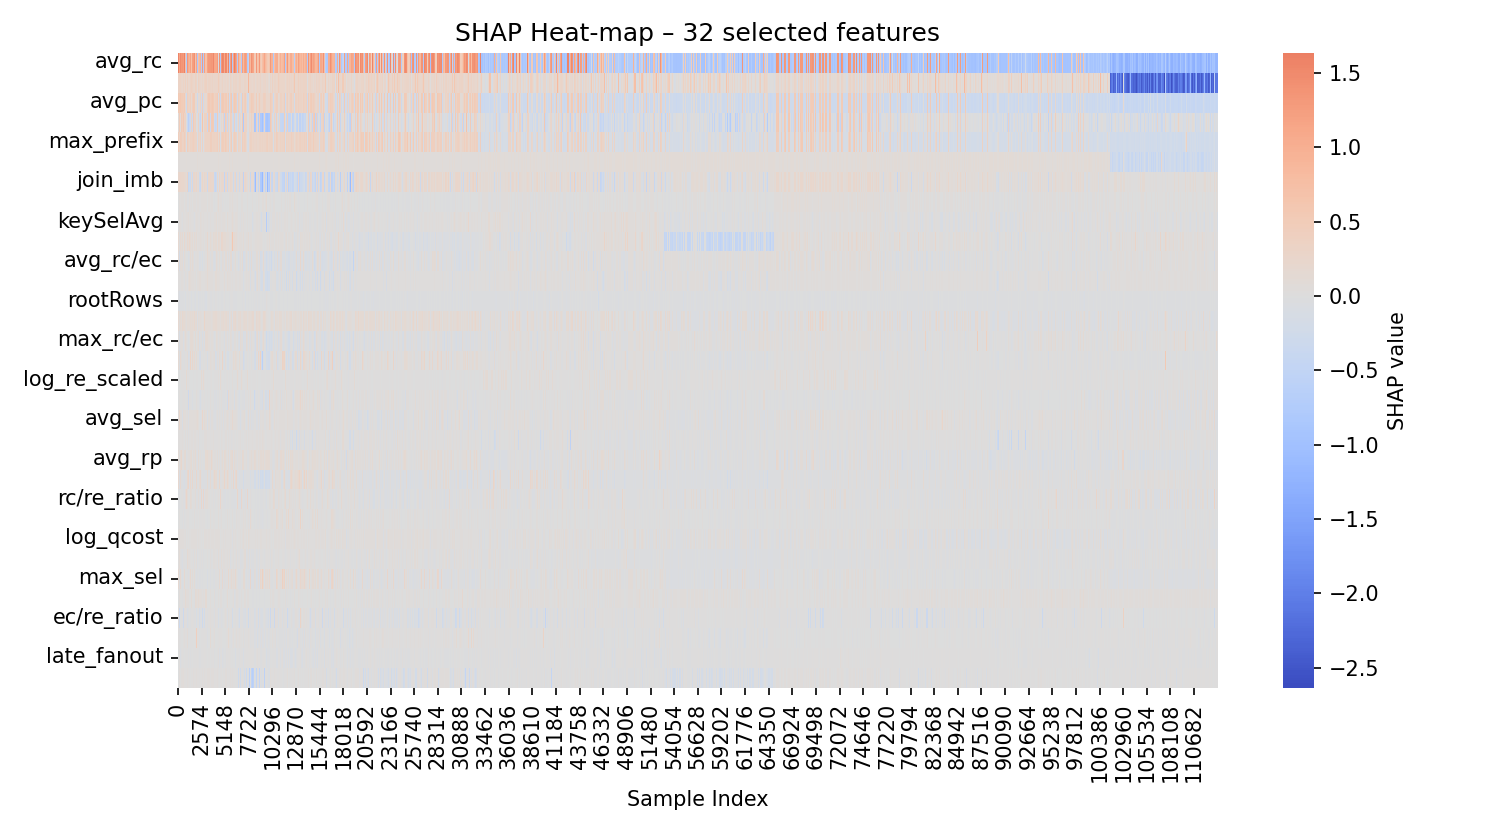
\includegraphics[width=\linewidth]{figures/shap_heatmap_top32.png}
    \caption{SHAP value heatmap: 16 of the selected 32 features. Darker colors indicate higher feature importance. Features are ordered by average importance.}
    \label{fig:heatmap}
    \vspace{-2em}
\end{figure}

Figure~\ref{fig:heatmap} visualizes the SHAP values of the top 16 of the 32 selected features as a heatmap, revealing that cost-related features (\texttt{avg\_rc}, \texttt{qcost/bytes}) and cardinality estimates (\texttt{rootRows}, \texttt{avg\_re}) rank among the most influential predictors. The complete list of selected features with their descriptions is provided in Appendix B\footnote{In the full version of this paper.}.



\subsection{Data Collection}\label{ssec:data_collection}

To construct a robust and representative training dataset that captures both widely adopted industry-standard benchmarks and realistic production workloads, we executed each query on both row-store and column-store engines, ensuring comprehensive performance labeling across diverse query characteristics and data distributions.
The public side of the workload comes from \textsc{TPC-H} and \textsc{TPC-DS} at scale factors 1, 10 and 100, and \textsc{hybench} at scale factors of 1 and 10. 
To keep the mix realistic we added seven production traces~\cite{hilprecht2022zero}: \textsc{Airline}, \textsc{Credit}, \textsc{Carcinogenesis}, \textsc{Employee}, \textsc{Financial}, \textsc{Geneea}, \textsc{Hepatitis}.

We generate query workloads by emulating real-world query patterns~\cite{hilprecht2022zero}. 
The workloads include queries with random joins adhering to schema definitions, predicates sampled from underlying data distributions (with a maximum of 20 predicates per query and a maximum of 10 joins), and complex logical expressions involving {AND} and {OR} operators. 
Additionally, queries incorporate aggregations with up to 3 operations and a maximum of 2 columns per aggregation, optional {GROUP BY} clauses (with a 20\% probability of including a {HAVING} condition), and {ORDER BY} clauses. 

All queries were executed on an instrumented PolarDB instance, from which we recorded the MySQL optimizer’s JSON plan, the actual runtimes of the row and column executions, and the relevant statistics. Each workload contributes at least 10K valid query samples, for a total of more than 150K labeled examples.



\subsection{Model Training}\label{ssec:model_training}

\subsubsection{Model Selection}
We evaluate four candidate models for query dispatch: CART (single decision tree)~\cite{loh2011classification}, Random Forest~\cite{breiman2001random}, feed-forward neural networks (FNN)~\cite{rumelhart1986learning,nissen2003fann}, and LightGBM~\cite{ke2017lightgbm}. Based on empirical results (Section~\ref{ssec:model-cmp}), we select LightGBM for its superior prediction accuracy and training efficiency.

\subsubsection{Training Objective}
We transform the binary classification problem into regression by using the log-difference target: $\log(\ell_{\text{row}}^i) - \log(\ell_{\text{col}}^i)$. This formulation naturally captures relative performance differences and improves gradient behavior. We use standard L2 regression loss with custom sample weighting (described below). Additionally, we compress gradients by 0.3× when the log-difference falls below 5\%, preventing overfitting to queries with similar execution times on both engines.



\subsubsection{Self-paced Taylor-weighted Boosting}\label{sssec:self_paced_boosting}

Standard uniform weigh-ting treats all training samples equally, but dispatch errors have asymmetric costs—mispredicting a query with large latency difference causes more harm than one with similar performance on both engines. We develop a novel sample weighting scheme motivated by Taylor expansion of the latency objective.
For a query with row latency $R$ and column latency $C$, the expected latency under probabilistic dispatch $p \in [0,1]$ is:
\(
T(p) = (1-p)R + pC = R + p(C-R)
\).
Taylor expansion around the optimal choice $p^* = \mathbb{1}_{\{C < R\}}$ yields:
\(
T(p) - T(p^*) \approx |C-R| \cdot |p-p^*| + \frac{1}{2}(C-R)^2 \cdot (p-p^*)^2
\).
The first-order term shows that misprediction cost scales linearly with the latency gap $|C-R|$, which motivates prioritizing queries with large performance differences.



\paragraph{Multi-Factor Weighting Scheme.}
Furthermore, we assign each training sample $i$ a weight that combines six factors:

\begin{enumerate}[leftmargin=*]
\item \textbf{Weight A - Class balance}: Inversely proportional to class frequency to handle label imbalance.

\item \textbf{Weight B - Gap amplification}: Proportional to $|\log(R_i/C_i)|$, emphasizing queries with large relative performance differences.

\item \textbf{Weight C - Dataset size}: Inversely proportional to $\sqrt{n_d}$ where $n_d$ is dataset size, preventing large datasets from dominating training.

\item \textbf{Weight D - Regret}: Proportional to $|R_i - C_i|$, directly from Taylor analysis—larger absolute latency differences receive higher weight.

\item \textbf{Weight E - Focal adjustment}: Proportional to $[1 - 2|p_i - 0.5|]^2$ where $p_i$ is model prediction. This emphasizes uncertain queries ($p_i \approx 0.5$) while down-weighting confident cases.

\item \textbf{Weight F - Runtime scale}: Proportional to $\min(R_i, C_i)^{\alpha}$ with $\alpha < 1$, giving more importance to slower queries.
\end{enumerate}

The final weight is the product of these factors, with soft clipping applied to prevent extreme values. The clipping bounds relax gradually across epochs to allow the model to focus on increasingly difficult examples.

\paragraph{Self-Paced Learning Procedure.}
After each epoch, we update each sample's predicted probability based on the current model. This creates a natural curriculum: early epochs treat all samples equally (since all start with $p_i = 0.5$), while later epochs automatically focus on challenging boundary cases where the model remains uncertain. This progression from uniform to focused learning improves robustness to noisy runtime measurements.

\subsubsection{Training Configuration}

\paragraph{Hyperparameters.}
Our LightGBM configuration balances model capacity with training efficiency:
\begin{itemize}[leftmargin=*,topsep=2pt,itemsep=1pt]
\item \textbf{Boosting}: GOSS (Gradient One-Side Sampling) for efficient large-scale training.
\item \textbf{Trees}: 400 per epoch, early stopping after 100 rounds without improvement.
\item \textbf{Tree structure}: max depth 18, up to 256 leaves, min 20 samples per leaf.
\item \textbf{Learning}: rate 0.045, decayed by 0.75× per epoch.
% \item \textbf{Sampling}: 80\% features, 70\% rows (plus 5\% GOSS).
\item \textbf{Regularization}: L2 weight 1.0, no L1 regularization.
% \item \textbf{Efficiency}: 127 histogram bins, 20 threads, validation every 10 iterations.
\end{itemize}

\paragraph{Cross-Validation and Ensemble.}
We employ 5-fold stratified cross-validation to ensure robust generalization. Each fold maintains the original class distribution and is trained independently with self-paced weighting. From the five resulting models, we select the top three by balanced accuracy on validation sets. During offline testing, these models form an ensemble with majority voting—queries dispatched to the column engine if more than half predict positive.



% ================================================================
\section{Online Dispatch}\label{sec:online}
% ================================================================

In this section, we describe the three stages of \emph{online dispatch} phase: \textit{LightGBM predicting}, \textit{residual learning}, and \textit{resource regulating}.

%------------------------------------------------------------------
\subsection{Stage\,1: LightGBM Predicting}\label{ssec:online_lgbm}


Each incoming query \(q_t\) is mapped to the
$d$-dimensional ($d=32$) feature vector
\(\mathbf x_t\) (see Section~\ref{ssec:feature_engineering}). 
LightGBM outputs a \emph{margin}
\(s_t \in \mathbb{R}\).
Using the logistic link
\(
 \pi_t \;=\; \sigma\!\bigl(s_t\bigr)
         \;=\;
         \frac{1}{1+e^{-s_t}}, 
\)
where \(\pi_t\) is the posterior probability that
\(q_t\) should be executed on the column engine (\textsf{AP}).


Rather than thresholding
\(\pi_t\) we pass the \emph{raw margin} \(s_t\) to the next stage:
its sign suggests the preferred engine,
while the magnitude encodes confidence
\cite{guo2017calibration}.
This continuous prior enables the residual learner
(Section~\ref{ssec:online_residual}) to focus exploration on
low-confidence or mispredicted queries.


%------------------------------------------------------------------
\subsection{Stage\,2: Residual Learning}\label{ssec:online_residual}

At time $t$ when a query finishes, we observe only the latency of the \emph{chosen} engine $\ell_{a_t}$. This creates a fundamental challenge: how can we learn whether the \emph{other} engine would have been faster without actually running the query on both engines.
To address this partial feedback problem, We maintain exponentially-weighted moving averages (EWMAs) of observed latencies for each engine\footnote{$\text{EWMA}_t=\alpha\ell_t+(1-\alpha)\text{EWMA}_{t-1}$ with smoothing factor $\alpha=0.03$.}: $\hat\lrow[t]$ and $\hat\lcol[t]$. These serve as \emph{counterfactual estimates} for the unobserved engine's performance.

we cast online adaptation as a \emph{linear contextual bandit} \cite{li2010contextual,abbasi2011improved} that learns to refine the base LightGBM predictions using streaming latency observations. We employ Thompson Sampling for exploration, which provides a principled probabilistic approach to the exploration-exploitation trade-off.


The \emph{signed residual} is constructed as below, where $\Delta_t$ is positive exactly when the column engine is (expected to be) faster. The logarithmic transformation ensures numerical stability and reduces the impact of latency outliers.
\begin{equation}\label{eq:residual}
    \Delta_t=
  \begin{cases}
    -\log(1+\ell_{col}[t]) + \log(1+\hat\ell_{row}[t]), & a_t=1\\[4pt]
    \log(1+\hat\ell_{col}[t]) - \log(1+\ell_{row}[t]), & a_t=0
  \end{cases}
\end{equation}
  
\subsubsection{LinTS-Delta: Bayesian Exploration for Runtime Adaptation}

We model the residual between predicted and actual engine performance as a linear function of query features: $\mathbb{E}[\Delta_t\mid\mathbf x_t]=\mathbf x_t^{\top}\boldsymbol\theta^\star$, where $\boldsymbol\theta^\star$ captures how query characteristics correlate with prediction errors.
LinTS-Delta employs Thompson Sampling~\cite{thompson1933likelihood,russo2018tutorial} to balance exploration and exploitation. The algorithm maintains a Bayesian posterior over $\boldsymbol\theta$ with regularization parameter $\lambda = 0.5$:
\(
V_t=\lambda I+\sum_{\tau=1}^{t}\mathbf{x}_{\tau}\mathbf{x}_{\tau}^{\top}, 
\mathbf{b}_t=\sum_{\tau=1}^{t}\mathbf{x}_{\tau}\Delta_{\tau}
\).
The posterior mean is $\hat{\boldsymbol{\theta}}_t = V_t^{-1}\mathbf{b}_t$ with covariance matrix $V_t^{-1}$. At each time step, we sample from this posterior distribution:
\(
\tilde{\boldsymbol{\theta}}_t \sim \mathcal{N}(\hat{\boldsymbol{\theta}}_{t-1}, \sigma^2 V_{t-1}^{-1})
\).
The Thompson score for the current query is then computed as:
\(
u_t = \mathbf x_t^{\top}\tilde{\boldsymbol{\theta}}_t
\).

This approach follows the linear contextual bandit framework~\cite{agrawal2013thompson,lattimore2020bandit}, where the covariance matrix $V_t^{-1}$ quantifies uncertainty about $\boldsymbol\theta$—high uncertainty (large eigenvalues of $V_t^{-1}$) induces exploration through diverse samples, while low uncertainty leads to exploitation.

% \paragraph{Integration with Learned Model.}
We then combine the static LightGBM prediction $s_t$ with the learned residual $u_t$ through:
\begin{equation}
z_t=\tanh(s_t+u_t)\in(-1,1)
\end{equation}

This fusion allows Thompson Sampling to refine rather than replace the base model, providing runtime adaptation while leveraging the strong baseline performance. The $\tanh$ function ensures bounded outputs suitable for downstream resource-aware dispatch.

\paragraph{Performance Guarantee.}
LinTS-Delta provides theoretical guarantees on its learning efficiency. The algorithm is proven to be a \emph{no-regret} learner, meaning it learns from its dispatch mistakes and improves over time. Specifically, after processing $T$ queries, the average extra latency caused by suboptimal dispatch decisions decreases proportionally to $\sqrt{1/T}$~\cite{lattimore2020bandit,russo2018tutorial}. This means the system gets twice as accurate when it sees four times more queries.


%------------------------------------------------------------------
\subsection{Stage\,3: Resource Regulating}\label{ssec:online_resource}

The first two stages favor the fastest engine, but production HTAP
systems must also respect CPU and memory budgets.  
In stage 3, our resource regulator tweaks the dispatch probability just
enough to keep the row/column engines “fairly level” over time. 
The steps are illustrated below:

\paragraph{Step 1 – Measure Utilization.}
After each query we record the row-engine share of resource utilization
\(
  \mathbf r_t = (\rho_t^{\text{cpu}},\rho_t^{\text{mem}})\in[0,1]^2.
\)

\paragraph{Step 2 – Compute an imbalance score.}
Let the instantaneous deviation of the row engine’s utilisation from
its target be
\begin{equation}
  \mathbf e_t \;=\;
     \mathbf r_t - \boldsymbol\gamma_t
   = \bigl(e_t^{\text{cpu}},\,e_t^{\text{mem}}\bigr)^{\!\top}\in\mathbb{R}^2 
\end{equation}


Periodically we recompute the empirical covariance matrix from the
\(K\) most recent deviations,
\begin{equation}
  \boldsymbol\Sigma_t \;=\;
  \frac{1}{K-1}\sum_{k=1}^{K}
      \bigl(\mathbf e_{t-k}-\bar{\mathbf e}\bigr)
      \bigl(\mathbf e_{t-k}-\bar{\mathbf e}\bigr)^{\!\top},
  \qquad
  \bar{\mathbf e}=\frac{1}{K}\sum_{k=1}^{K}\mathbf e_{t-k},
\end{equation}
which, in two dimensions, expands to
\begin{equation}
  \boldsymbol\Sigma_t
    \;=\;
    \begin{pmatrix}
      s_{\text{cpu}}^{2} & s_{\text{cpu,mem}} \\
      s_{\text{cpu,mem}} & s_{\text{mem}}^{2}
    \end{pmatrix},
\end{equation}
where
\begin{equation}
    s_{\text{cpu}}^{2}
    = \operatorname{Var}\!\bigl[e^{\text{cpu}}\bigr], \quad
  s_{\text{mem}}^{2}
    = \operatorname{Var}\!\bigl[e^{\text{mem}}\bigr], \quad
  s_{\text{cpu,mem}}
    = \operatorname{Cov}\!\bigl[e^{\text{cpu}},e^{\text{mem}}\bigr].
\end{equation}
  



We measure the imbalance magnitude with the Mahalanobis distance~\cite{mclachlan1999mahalanobis} and
attach a sign based on the CPU deviation:
\begin{equation}
\begin{split}
  d_t
  &= \operatorname{sgn}\!\bigl(e_t^{\text{cpu}}\bigr)\,
     \sqrt{\mathbf e_t^{\top}\,\boldsymbol\Sigma_t^{-1}\,\mathbf e_t} \\[2pt]
  &= \operatorname{sgn}\!\bigl(e_t^{\text{cpu}}\bigr)\,
     \sqrt{\frac{(e_t^{\text{cpu}})^2 s_{\text{mem}}^{2}
                 \;-\; 2 e_t^{\text{cpu}} e_t^{\text{mem}} s_{\text{cpu,mem}}
                 \;+\; (e_t^{\text{mem}})^2 s_{\text{cpu}}^{2}}
                {s_{\text{cpu}}^{2}s_{\text{mem}}^{2}-s_{\text{cpu,mem}}^{2}} } .
\end{split}
\end{equation}


Finally we squash the signed distance to \([-1,1]\):
\[
  r_t \;=\; \tanh(d_t),
\]
so that positive values indicate the row engine is
\emph{over‑utilizing} CPU/MEM relative to its target
(\(e_t^{\text{cpu}}>0\)), while negative values indicate
\emph{under‑utilization}.




\paragraph{Step 3 – Fuse speed and resource signals.}
Recall $z_t\in(-1,1)$ from Phase 2
(positive $\Rightarrow$ column engine predicted faster).
We mix the two scores:
\[
  s^{\text{final}}_t
  \;=\;
  \omega_t\,z_t \;+\; (1-\omega_t)\,r_t,
\quad
  \omega_t = 
    0.4 + 0.3 \cdot
    \sigma\!\bigl(\hat\lambda_t/5-1\bigr),
\]
where \(\hat{\lambda}_t\) is the current QPS estimate and \(\sigma(x) = 1/(1 + e^{-x})\).  
\begin{itemize}[leftmargin=*]
  \item Low load (QPS \(\approx 0\)) \(\Rightarrow\) \(\omega_t \approx 0.481\)  
    \(\rightarrow\) prioritize resource parity.
  \item High load (QPS \(\to +\infty\)) \(\Rightarrow\) \(\omega_t \approx 0.7\)  
    \(\rightarrow\) prioritize latency.
\end{itemize}

Dispatch to the column engine iff $s^{\text{final}}_t>0$.

\paragraph{Step 4 – Update the target using a simple OCO move.}
Periodically we look at the current resource error  
$g_t := \mathbf r_t - \boldsymbol\gamma_t$  
and run an Online-Convex-Optimization (OCO)~\cite{zinkevich2003online} step on the target share:

\begin{equation}
  \boldsymbol\gamma_{t+1}
  \;=\;
  \Pi_{[0,1]^2}\!
  \bigl(
     \boldsymbol\gamma_t - \beta\, g_t
  \bigr),
  \qquad
  \beta = \frac{c}{\sqrt{t}}\;(c>0).
\end{equation}

\noindent
Here $\Pi_{[0,1]^2}$ is the projection operator:
it simply clips each coordinate so the target stays in the box
$[0,1]^2$ (that is, never below 0 or above 1).

\begin{itemize}[leftmargin=*]
  \item \textbf{Column repeatedly wins on speed.}  
        Suppose over the last 30s the column engine is almost always
        faster than the row engine.  
        In that case the row engine’s CPU/MEM share
        $\mathbf r_t$ is “too high for its performance,” so  
        $g_t = \mathbf r_t-\boldsymbol\gamma_t$ is \emph{positive}.  
        The update
        $\boldsymbol\gamma_{t+1}
          = \boldsymbol\gamma_t - \beta\,g_t$
        therefore \emph{reduces} the row-engine target and gives a
        larger share to the column engine for the next window.

  \item \textbf{Row engine is short on resources.}  
        If monitoring shows the row engine now has \emph{less} CPU/MEM
        than its target, then
        $\mathbf r_t$ drops below $\boldsymbol\gamma_t$
        and $g_t$ becomes \emph{negative}.  
        The same update rule
        $\boldsymbol\gamma_{t+1}
           = \boldsymbol\gamma_t - \beta\,g_t$
        now \emph{increases} the row-engine target, asking the
        dispatcher to send more queries its way and restore balance.
\end{itemize}


\subsection{Online Query Dispatch Algorithm}
Algorithm~\ref{alg:LCDispatcher} integrates three stages of online query dispatch with continuous adaptation. After initialization (Lines 2-6), each query $q_t$ is processed as follows: Stage 1 extracts features $\mathbf{x}_t$ and computes base score $s_t$ via LightGBM (Lines 8-9). Stage 2 applies Thompson Sampling to generate residual adjustment $u_t$, yielding latency score $z_t = \tanh(s_t + u_t)$ (Lines 10-12). Stage 3 tracks resource deviation $\mathbf{e}_t$ and computes normalized Mahalanobis distance $r_t$ for resource balancing (Lines 13-23). The final score $s_t^{\text{final}} = \omega_t z_t + (1-\omega_t) r_t$ uses load-adaptive weighting $\omega_t$, with positive values selecting the column engine (Lines 24-26). Post-execution, the algorithm updates EWMA latencies, LinTS posterior using log-residual rewards, and resource targets via online convex optimization (Lines 28-33).


\begin{algorithm}[t]
\caption{\textsc{\dispatcher}: Unified online adaptive dispatch with Thompson Sampling \& Mahalanobis balancing}
\label{alg:LCDispatcher}
\begin{algorithmic}[1]
\Require LightGBM model $f$ (offline–trained); LinTS hyper‑parameters $(\lambda,\sigma^{2})$;  
         OCO step‑size constant $c$; update period $S$ (seconds); buffer length $K$
\Ensure Engine choice $a_t\in\{0,1\}$ for every incoming query $q_t$
\State \textbf{Initialise:}
\State \hspace{1em}$V\leftarrow\lambda I_d$,  $\mathbf b\leftarrow\mathbf 0$ \Comment{LinTS posterior stats}
\State \hspace{1em}$\hat\ell^{\mathrm{row}}\!\leftarrow0$, $\hat\ell^{\mathrm{col}}\!\leftarrow0$ \Comment{EWMA latencies}
\State \hspace{1em}$\boldsymbol\gamma_1\!\leftarrow(0.5,0.5)$ \Comment{row‑engine CPU/MEM target}
\State \hspace{1em}$\boldsymbol\Sigma_1\!\leftarrow I_2$,\; $\mathcal B\leftarrow\varnothing$ \Comment{covariance, buffer}
\State \hspace{1em}\textit{lastCov} $\leftarrow$\Call{Now}{},\;
                 \textit{lastOCO} $\leftarrow$\Call{Now}{}
\For{\textbf{each} query $q_t$ arriving at time $t$}
  %---------------- Phase 1 --------------------------------------------------
  \State /* \textbf{Stage 1 – LightGBM Predicting} */
  \State $\mathbf x_t\!\leftarrow$\Call{ExtractFeatures}{$q_t$};\;
        $s_t\!\leftarrow f(\mathbf x_t)$
  %---------------- Phase 2 --------------------------------------------------
  \State /* \textbf{Stage 2 – Residual Learning} */
  \State sample $\tilde{\boldsymbol\theta}_t\!\sim\mathcal N(V^{-1}\mathbf b,\sigma^{2}V^{-1})$
  \State $u_t\!\leftarrow\mathbf x_t^{\!\top}\tilde{\boldsymbol\theta}_t$;\;
        $z_t\!\leftarrow\tanh(s_t+u_t)$        \Comment{$z_t\in(-1,1)$}
  %---------------- Phase 3 --------------------------------------------------
  \State /* \textbf{Stage 3 – Resource Regulating} */
  \State $\mathbf r_t\!\leftarrow(\rho_t^{\mathrm{cpu}},\rho_t^{\mathrm{mem}})$
  \State $\mathbf e_t\!\leftarrow\mathbf r_t-\boldsymbol\gamma_t$        
  \State append $\mathbf e_t$ to $\mathcal B$ and drop oldest if $|\mathcal B|>K$
  \If{$\Call{Now}{}-\textit{lastCov}\ge S$}
     \State $\boldsymbol\Sigma_t\leftarrow\mathrm{COV}(\mathcal B)$
     \State \textit{lastCov}$\leftarrow$\Call{Now}{}
  \EndIf
  \State $d_t\!\leftarrow
          \operatorname{sgn}(e_t^{\mathrm{cpu}})
          \sqrt{\mathbf e_t^{\!\top}\boldsymbol\Sigma_t^{-1}\mathbf e_t}$
  \State $r_t\!\leftarrow\tanh(d_t)$
  \State $\omega_t\!\leftarrow0.4+0.3\cdot\sigma(\hat\lambda_t/5-1)$
  \State $s^{\mathrm{final}}_t\!\leftarrow\omega_t z_t+(1-\omega_t) r_t$
  \State $a_t\!\leftarrow\mathbf 1\!\left[s^{\mathrm{final}}_t>0\right]$\,
         \Comment{$1$: column, $0$: row}
  %---------------- Execute & observe ---------------------------------------
  \State $\ell_{a_t}\!\leftarrow$\Call{Execute}{$q_t,a_t$} \Comment{actual latency}
  %---------------- LinTS posterior update ----------------------------------
  \State $\hat\ell^{(a_t)}\!\leftarrow
           \alpha\,\ell_{a_t}+(1-\alpha)\,\hat\ell^{(a_t)}$ \Comment{update EWMA latency}
  \State \[
          \Delta_t =
          \begin{cases}
            -\log\!\bigl(1+\ell_{a_t}\bigr) +
            \log\!\bigl(1+\hat\ell^{\mathrm{row}}\bigr), & a_t=1 \\[4pt]
            -\log\!\bigl(1+\hat\ell^{\mathrm{col}}\bigr) +
            \log\!\bigl(1+\ell_{a_t}\bigr), & a_t=0
          \end{cases}
        \] \Comment{residual reward}
  \State $V\leftarrow V+\mathbf x_t\mathbf x_t^{\!\top}$;\;
        $\mathbf b\leftarrow\mathbf b+\mathbf x_t\,\Delta_t$
  %---------------- OCO move for $\gamma$ -----------------------------------
  \If{$\Call{Now}{}-\textit{lastOCO}\ge S$}
     \State $\beta_t\leftarrow c/\sqrt{t}$
     \State $\boldsymbol\gamma_{t+1}\leftarrow
            \Pi_{[0,1]^2}\!\bigl[\boldsymbol\gamma_t
               -\beta_t(\mathbf r_t-\boldsymbol\gamma_t)\bigr]$
     \State \textit{lastOCO}$\leftarrow$\Call{Now}{}
  \EndIf
\EndFor
\end{algorithmic}
\end{algorithm}

%------------------------------------------------------------------
\subsection{Performance Guarantee}
\label{sssec:perf_guarantee}
\dispatcher provides theoretical guarantees on both latency optimization and resource balance:


\begin{theorem}[]
\label{thm:perf}
Let a horizon of \(T\) queries be served by the three-phase pipeline
described in
Sections~\ref{ssec:online_lgbm}–\ref{ssec:online_resource}.
Assume:
\begin{enumerate}
\item \textbf{bounded latency:} \(\max_{t}\ell_{a_t}\le L_{\max}\);
\item \textbf{bounded resources:} \(\|\mathbf r_t\|_2\le 1\;\forall t\);
\item \textbf{weight constraint:} the scalar weight satisfies
      \(\alpha_t\ge 0.48\;\forall t\).
\end{enumerate}
Then there exists constants \(C_1>0\) and \(C_2>0\) such that
\begin{equation}
    \frac1T\sum_{t=1}^{T}
  \bigl(\ell_{t}(a_t)-\min_{a}\ell_{t}(a)\bigr)
\le
  \frac{C_1\,\sqrt{\log T}}{\sqrt{T}},
   \label{eq:perf_speed}
\end{equation}


\begin{equation}
\frac{1}{T}\sum_{t=1}^{T}
  \bigl\|\mathbf{r}_t-\boldsymbol{\gamma}_t\bigr\|_2^{2}
\le
  \frac{C_2}{\sqrt{T}}.
\label{eq:perf_resource}
\end{equation}


Equation~\eqref{eq:perf_speed} bounds the \emph{average extra latency}
with respect to the optimal; \eqref{eq:perf_resource} bounds the
\emph{average squared resource drift} relative to the adaptive target
\(\boldsymbol\gamma_t\).
\end{theorem}

The proof sketch of Theorem~\ref{thm:perf} is shown in Appendix C\footnote{In the full version of this paper.}.



%%%%%%%%%%%%%%%%%%%%%%%%%%%%%%%%%%%%%%%%%%%%%%%%%%%%%%%%%%%%%%%%%%%%%%%%%%
\section{Experimental Evaluation}
\label{sec:exp}

We evaluate \dispatcher through comprehensive experiments covering both offline model training and online query dispatch under varying concurrency levels.

\subsection{Experimental Setup}
\paragraph{Hardware.}
All experiments run on a dual-socket server equipped with two Intel\textsuperscript{\textregistered} Xeon Platinum 8269CY processors (26 cores, 52 threads each, base 2.5 GHz, turbo 3.8 GHz) and 768\,GB DDR4 RAM. % The machine has 104 logical CPUs.

\vspace{-0.8em}

\paragraph{Implementation.}
\dispatcher is fully integrated into PolarDB at the kernel level. The dispatcher is implemented in modern C++, linking against the native LightGBM C API for inference~\cite{ke2017lightgbm}. The trained model (approximately 10\,MB) is loaded by the engine. Feature extraction and inference combined add about 500 $\mu s$ overhead per query.

\subsection{Baselines}

We compare two variants of \dispatcher (LightGBM Static and LightGBM Dynamic) against four representative approaches:

\begin{enumerate}[leftmargin=*,itemsep=2pt]
  \item \textbf{Row-only}: Dispatches all queries to the row engine.
  \item \textbf{Column-only}: Dispatches all queries to the column engine.
  \item \textbf{Cost-threshold}: PolarDB's default strategy—dispatches to column engine when optimizer cost exceeds $5\times10^{4}$, otherwise to row engine.
  \item \textbf{Hybrid Optimizer}: Uses linear regression to map optimizer costs to actual runtimes, then selects the engine with lower predicted latency~\cite{PolarDBHybridOptimizerBlog}.
\end{enumerate}

LightGBM Static only uses the prediction from offline trained LightGBM model to dispatch queries, while LightGBM Dynamic includes residual learning and resource regulating.

Additionally, we evaluate three ML-based alternatives (Decision Tree, Random Forest, Feed-forward Neural Network) in Section~\ref{ssec:model-cmp} to validate our choice of LightGBM.


\subsection{Evaluation Metrics}
We employ different metrics for offline and online evaluation phases:

\paragraph{Metrics for Query-Level Dispatch}
We evaluate query-level dispatch using several metrics: (1) \textbf{Prediction Quality} measures standard classification metrics including accuracy, macro-precision, macro-recall, and macro-F$_1$ score, with separate F$_1$ scores reported for "easy" queries (where cost-threshold is correct) and "hard" queries (where cost-threshold is wrong); (2) \textbf{Average Runtime} measures the average runtime across all queries in a workload in seconds; (3) \textbf{Overall Improvement} captures the relative latency reduction compared to the cost-threshold baseline, calculated as $\text{improvement} = \frac{\text{avg-rt}_{\text{cost-thr}} - \text{avg-rt}_{\text{method}}}{\text{avg-rt}_{\text{cost-thr}}}$; and (4) \textbf{Improvement $\to$ Optimal} represents the fraction of theoretically achievable improvement captured, computed as $\frac{\text{avg-rt}_{\text{cost-thr}} - \text{avg-rt}_{\text{method}}}{\text{avg-rt}_{\text{cost-thr}} - \text{avg-rt}_{\text{optimal}}}$.

\paragraph{Metrics for Workload-Level Dispatch}
For workload-level dispatch evaluation, we track: (1) \textbf{Makespan}, the total wall-clock time from first query arrival to last query completion, which captures system throughput under load; (2) \textbf{Average Latency}, measuring the mean per-query execution time under concurrent load; (3) \textbf{P95 Latency}, the 95th percentile query latency that indicates tail behavior; and (4) \textbf{Resource Utilization}, tracking CPU percentage and memory consumption separately for row and column engines to measure resource balance and efficiency.


\subsection{Offline Preparation}
We first evaluate the offline LightGBM model's ability to predict optimal engine selection without runtime adaptation.

\subsubsection{Single-Dataset Results}
\label{sssec:single-ds}

Across the 15 workloads in Table~\ref{tab:single-ds},
\textbf{LightGBM delivers the lowest latency on 14 of them}.
Relative to the cost-threshold rule it trims runtime by a
\emph{median 17\,\%}, reaching
54\,\% on \texttt{tpch100},
44\,\% on \texttt{airline},
65\,\% on \texttt{employee}.
It improves over cost-threshold method up to 99\% towards the optimal.
Accuracy remains strong ($\ge0.85$ on 11 workloads).
The only outlier is the highly imbalanced \texttt{credit} trace, where
the column engine alone is 5\,\% faster than LightGBM, yet the model
still beats the cost rule by 17\,\%.
F$_1$ is mostly above 0.9 for “easy” queries (the cost-threshold method predicts them correctly), and has improvement over the cost-threshold method on "hard" queries (the cost threshold method misclassifies them).



\begin{table*}[!h]
  \centering
  \small
  \setlength{\tabcolsep}{4pt}
  \caption{Prediction quality and average runtime (s) on individual datasets.\\
  \footnotesize{$\uparrow$ = higher is better; $\downarrow$ = lower is better.}}
  \label{tab:single-ds}
  \resizebox{\textwidth}{!}{%
  \begin{tabular}{l *{15}{S[table-format=1.4]}}
    \toprule
    & \multicolumn{15}{c}{\textbf{Dataset}} \\
    \cmidrule(lr){2-16}
    \textbf{Metric} $\uparrow\!/\!\downarrow$ &
      \texttt{tpch1} &
      \texttt{tpch10} &
      \texttt{tpch100} &
      \texttt{tpcds1} &
      \texttt{tpcds10} &
      \texttt{tpcds100} &
      \texttt{hybench\_sf1} &
      \texttt{hybench\_sf10} &
      \texttt{airline} &
      \texttt{credit} &
      \texttt{carcinogenesis} &
      \texttt{employee} &
      \texttt{financial} &
      \texttt{geneea} &
      \texttt{hepatitis} \\ \midrule
%
    row avg-rt $\downarrow$            & 5.4970 & 21.016 &  8.4372 & 4.4619 & 10.4921 & 18.3224 & 2.5789 & 8.3067 & 0.1371 & 3.8453 & 0.0364 & 0.1367 & 0.5373 & 0.3610 & \textbf{0.0023} \\
    col avg-rt $\downarrow$            & 0.9219 &  3.987 &  6.8619 & 0.5928 &  2.0995 &  3.0967 & 0.6385 & 2.0188 & 0.0802 & \textbf{0.6044} & 0.0195 & 0.0368 & 0.0911 & 0.1351 & 0.0378 \\
    cost-thr. avg-rt $\downarrow$      & 0.9248 &  4.109 &  6.9390 & 0.5944 &  2.3815 &  3.2861 & 0.5955 & 1.8997 & 0.0628 & 0.7663 & 0.0149 & 0.0636 & 0.1001 & 0.1183 & \textbf{0.0023} \\
    hybrid avg-rt $\downarrow$         & 0.9616 &  4.414 &  7.6116 & 0.6028 &  2.3927 &  3.5906 & 0.8604 & 2.9427 & 0.0621 & 0.6347 & 0.0237 & 0.0335 & 0.2100 & 0.1278 & 0.0217 \\
    \textbf{LightGBM avg-rt} $\downarrow$  & \textbf{\num{0.9206}} &  \textbf{4.036} & \textbf{3.1683} & \textbf{0.5872} & \textbf{2.1460} & \textbf{3.1795} & \textbf{0.5609} & \textbf{1.7424} & \textbf{0.0350} & 0.6361 & \textbf{0.0109} &
                                          \textbf{0.0223} & \textbf{0.0826} & \textbf{0.1139} & \textbf{0.0023} \\
    optimal avg-rt $\downarrow$        & 0.9008 &  3.830 &  2.7906 & 0.5637 &  1.6681 &  2.2593 & 0.5176 & 1.5222 & 0.0307 & 0.5857 & 0.0108 & 0.0218 & 0.0810 & 0.1066 & \textbf{0.0023} \\ \addlinespace \midrule
%
    accuracy $\uparrow$                & 0.8677 & 0.8584 & 0.9309 & 0.7840 & 0.7917 & 0.8106 & 0.8965 & 0.8921 & 0.9323 & 0.7275 & 0.9668 & 0.9892 & 0.9376 & 0.9335 & 0.9997 \\
    macro precision $\uparrow$         & 0.8393 & 0.8276 & 0.8817 & 0.7296 & 0.6965 & 0.7666 & 0.8967 & 0.8873 & 0.8138 & 0.5298 & 0.6598 & 0.9803 & 0.7303 & 0.7320 & 0.4998 \\
    macro recall $\uparrow$            & 0.9879 & 0.9547 & 0.8367 & 0.9662 & 0.9444 & 0.9110 & 0.8849 & 0.8728 & 0.8701 & 0.9585 & 0.8889 & 0.9956 & 0.9420 & 0.8466 & 0.50 \\
    macro F$_1$ $\uparrow$             & 0.9076 & 0.8867 & 0.8586 & 0.8314 & 0.8017 & 0.8326 & 0.8899 & 0.8792 & 0.8410 & 0.6824 & 0.7574 & 0.9879 & 0.8228 & 0.7851 & 0.4999 \\ \addlinespace
%
    F$_1$ (easy) $\uparrow$            & 0.9863 & 0.9804 & 0.9222 & 0.9569 & 0.9520 & 0.9347 & 0.9406 & 0.9239 & 0.8731 & 0.6741 & 0.1778 & 0.9619 & 0.8264 & 0.7948 & 0.50 \\
    F$_1$ (hard) $\uparrow$            & 0.6609 & 0.5244 & 0.2286 & 0.4719 & 0.3289 & 0.4478 & 0.6992 & 0.7424 & 0.8000 & 0.6918 & 0.9677 & 0.9957 & 0.8108 & 0.7829 & 0.00 \\ \addlinespace \midrule
%
    overall impr. $\uparrow$           & 0.0045 & 0.0177 & 0.5434 & 0.0122 & 0.0989 & 0.0324 & 0.0581 & 0.0828 & 0.4431 & 0.1699 & 0.2659 & 0.6491 & 0.1748 & 0.0376 & 0.00 \\
    impr.\ $\to$ optimal $\uparrow$    & 0.1722 & 0.2609 & 0.9089 & 0.2360 & 0.3302 & 0.1038 & 0.4439 & 0.4168 & 0.8677 & 0.7209 & 0.9700 & 0.9867 & 0.9153 & 0.3797 & 0.00 \\
    \bottomrule
  \end{tabular}}
  \vspace{0.2em}
  \footnotesize{\textbf{Note:} Bold values indicate the best performance among row-only, column-only, cost threshold, hybrid optimizer, and LightGBM methods.}
\end{table*}



\subsubsection{Cross-Dataset Test}
\label{sssec:cross_dataset}

To test the model's generalization across datasets, we conduct a
\emph{leave-three-datasets-out} study.
The fifteen datasets are partitioned into five disjoint test groups  
(each group contains three datasets and appears exactly once as the
\emph{unseen} test set; the remaining twelve are used for training).

Table \ref{tab:x-ds} summarizes the results.  
Against MySQL’s \emph{cost-threshold} rule (our baseline for
\emph{improvement}), LightGBM reduces mean latency by
\textbf{42 \%}, \textbf{14 \%}, \textbf{13 \%}, \textbf{43 \%}, and
\textbf{22 \%} on the five splits, reclaiming \textbf{87 \%},
\textbf{75 \%}, \textbf{65 \%}, \textbf{81 \%}, and \textbf{71 \%} of the
oracle’s headroom while keeping accuracy mostly around 90\%. 
LightGBM achieves f1 score over 0.79 on all test sets.

\begin{table*}[t]
  \centering
  \small
  \setlength{\tabcolsep}{4pt}
  \caption{Cross-dataset evaluation.  Each row trains on twelve datasets
           and tests on the three unseen datasets shown in
           \textbf{Test Set}.  
           $\uparrow$\,/\,$\downarrow$ indicate the desired direction.}
  \label{tab:x-ds}
  \resizebox{\textwidth}{!}{
  \begin{tabular}{
      l
      S[table-format=1.6]
      S[table-format=1.6]
      S[table-format=1.6]
      S[table-format=1.6]
      S[table-format=1.6]
      S[table-format=1.6]
      S[table-format=1.3]
      S[table-format=1.3]
      S[table-format=1.3]
      S[table-format=1.3]}
    \toprule
    \textbf{Test Set} &
    {\footnotesize row avg-rt$\downarrow$} &
    {\footnotesize col avg-rt$\downarrow$} &
    {\footnotesize cost-thr. avg-rt$\downarrow$} &
    {\footnotesize hybrid avg-rt$\downarrow$} &
    {\footnotesize LightGBM avg-rt$\downarrow$} &
    {\footnotesize oracle avg-rt$\downarrow$} &
    {\footnotesize acc$\uparrow$} &
    {\footnotesize macro F$_1$$\uparrow$} &
    {\footnotesize overall impr.$\uparrow$} &
    {\footnotesize impr.$\!\to$oracle$\uparrow$} \\
    \midrule
    tpcds\_sf10 + hybench\_sf10 + tpch\_sf100 &
      6.46006 & 2.34585 & 2.27190 & 2.79300 & 1.31939 & 1.17715 &
      0.89385 & 0.89333 & 0.41926 & 0.87007 \\
    carcinogenesis + employee + hybench\_sf1 &
      0.97819 & 0.25657 & 0.24842 & 0.33530 & 0.21496 & 0.20356 &
      0.91766 & 0.91552 & 0.13471 & 0.74597 \\
    tpch\_sf1 + airline + hepatitis &
      1.26544 & 0.18964 & 0.18483 & 0.24029 & 0.16118 & 0.14831 &
      0.91837 & 0.90091 & 0.12795 & 0.64761 \\
    tpch\_sf10 + credit + tpcds\_sf100 &
      2.13144 & 0.63315 & 0.66784 & 0.77345 & 0.38044 & 0.31179 &
      0.80214 & 0.79197 & 0.43033 & 0.80717 \\
    tpcds\_sf1 + geneea + financial &
      0.65928 & 0.11423 & 0.11844 & 0.12394 & 0.09199 & 0.08130 &
      0.90223 & 0.87273 & 0.22329 & 0.71217 \\
    \bottomrule
  \end{tabular}
  }
\end{table*}



\begin{table}[t]
  \centering
  \small
  \setlength{\tabcolsep}{3.5pt}
  \caption{Comparison among Different AI Models}
  \label{tab:model-cmp}
  \resizebox{\linewidth}{!}{%
  \begin{tabular}{@{}lcccc@{}}
    \toprule
    \textbf{Metric} & \textbf{LightGBM} & \textbf{Random Forest} & \textbf{Decision Tree} & \textbf{FNN} \\
    \midrule
    Avg. runtime (ms) $\downarrow$     & \textbf{2.41} & 2.86 & 4.10 & 4.21 \\
    Accuracy $\uparrow$                & \textbf{0.91} & 0.78 & 0.42 & 0.49 \\
    Macro F$_1$ $\uparrow$             & \textbf{0.91} & 0.78 & 0.30 & 0.43 \\
    F$_1$ (hard) $\uparrow$            & \textbf{0.72} & 0.46 & 0.12 & 0.27 \\
    Overall impr. $\uparrow$      & \textbf{41.5\%} & 30.5\% & 0.5\% & –2.1\% \\
    Impr. $\to$ optimal $\uparrow$ & \textbf{96.8\%} & 71.1\% & 1.3\% & –4.8\% \\
    \bottomrule
  \end{tabular}%
  }
  \vspace{-1em}
\end{table}


% --------------------------------------------------------
\subsubsection{Model Comparison}
\label{ssec:model-cmp}
% \textcolor{red}{add gnn model in this section }
To evaluate the impact of the learning algorithm itself, we train four
classifiers—LightGBM, Random Forest (RF), a single Decision-Tree
(DT), and feed forward neural network (FNN) —on the \emph{same} features and
training data.  
Table~\ref{tab:model-cmp} compares their performance.

LightGBM delivers the lowest average runtime (\textbf{2.41 ms}),
exceeding the cost-threshold rule by \textbf{41.5 \%} and recovering
\textbf{96.8 \%} of the optimal’s headroom, while maintaining the highest
macro-F\(_1\) and hard-query F\(_1\).  
RF provides a moderate gain but is 18\% slower than LightGBM.
Both DT and FNN fail to improve much over the heuristic baseline.


% --------------------------------------------------------
\subsubsection{Ablation Study}
\label{sec:ablation}

We ablate two implementation knobs—\emph{hard-example replay} and the six
sample-weight terms \emph{A–F} introduced in
Section~\ref{sssec:self_paced_boosting} — by disabling them one at a time.
Turning off any single component hurts both runtime and quality,
showing that each contributes additively.  
Hard-example replay is the most influential: removing it raises mean
latency by \(+3.2\%\) and lowers macro-F\(_1\) by 0.032, while the
hard-query F\(_1\) drops from 0.646 to 0.586. The detailed results are shown in Appendix D\footnote{In the full version of this paper.}.


\subsection{Online Dispatch}
\label{subsec:online-dispatch}

We now evaluate \dispatcher's performance under concurrent query execution, where runtime adaptation becomes critical for handling dynamic workloads and resource contention in production environments. The generation of the queries is described in Section~\ref{ssec:data_collection}.

\subsubsection{Comparison between Four Dispatch Methods}
\label{subsubsec:static-vs-dynamic}
To isolate the benefits of online adaptation, we conduct a comprehensive evaluation comparing four dispatch strategies under increasing concurrency levels from 200 to 1000 concurrent queries. The \texttt{Cost Threshold} and \texttt{Hybrid Optimizer} represent state-of-the-art rule-based approaches currently deployed in production systems~\cite{wang2023polardb}, while \texttt{LightGBM Static} employs our offline-trained gradient boosting model without runtime adaptation. The \texttt{LightGBM Dynamic} variant incorporates our novel LinTS-Delta algorithm, combining Bayesian exploration with resource-aware regulation to address the exploration exploitation tradeoff in online settings.


\begin{table}[t]
\centering
\caption{Performance Comparison of Dispatch Strategies under Varying Concurrency Levels.}
\label{tab:routing_perf}
\resizebox{\columnwidth}{!}{%
\begin{tabular}{@{}lccc@{}}
\toprule
\textbf{Dispatch Strategy} & \textbf{Makespan (s)$\downarrow$} & \textbf{Avg Latency (s)$\downarrow$} & \textbf{P95 Latency (s)$\downarrow$} \\
\midrule
\multicolumn{4}{c}{\textit{200 Concurrent Queries}} \\
\midrule
Cost Threshold     & 127.11   & 1.65   & 6.94   \\
Hybrid Optimizer   & 126.45   & 1.62   & 6.57   \\
LightGBM Static    & 20.42    & 0.49   & 1.62   \\
LightGBM Dynamic   & \textbf{19.49}    & \textbf{0.42}   & \textbf{1.36}   \\
\hdashline
\textit{Improvement} & 84.7\% & 74.4\% & 80.5\% \\
\midrule
\multicolumn{4}{c}{\textit{400 Concurrent Queries}} \\
\midrule
Cost Threshold     & 126.61   & 1.22   & 4.37   \\
Hybrid Optimizer   & 125.80   & 1.33   & 5.56   \\
LightGBM Static    & 22.88    & 0.58   & 2.70   \\
LightGBM Dynamic   & \textbf{22.45}    & \textbf{0.52}   & \textbf{1.61}   \\
\hdashline
\textit{Improvement} & 82.3\% & 57.0\% & 63.1\% \\
\midrule
\multicolumn{4}{c}{\textit{600 Concurrent Queries}} \\
\midrule
Cost Threshold     & 126.44   & 1.19   & 5.14   \\
Hybrid Optimizer   & 126.92   & 1.27   & 4.97   \\
LightGBM Static    & 44.36    & 0.77   & 3.11   \\
LightGBM Dynamic   & \textbf{38.67}    & \textbf{0.67}   & \textbf{2.64}   \\
\hdashline
\textit{Improvement} & 69.4\% & 43.9\% & 48.6\% \\
\midrule
\multicolumn{4}{c}{\textit{800 Concurrent Queries}} \\
\midrule
Cost Threshold     & 125.83   & 2.10   & 9.19   \\
Hybrid Optimizer   & 126.49   & 1.77   & 8.16   \\
LightGBM Static    & 83.43    & 1.29   & 4.94   \\
LightGBM Dynamic   & \textbf{74.50}    & \textbf{1.14}   & \textbf{4.56}   \\
\hdashline
\textit{Improvement} & 40.8\% & 45.8\% & 50.4\% \\
\midrule
\multicolumn{4}{c}{\textit{1000 Concurrent Queries}} \\
\midrule
Cost Threshold     & 137.36   & 3.74   & 16.07   \\
Hybrid Optimizer   & 125.86   & 2.91   & 11.84   \\
LightGBM Static    & 113.59   & 1.73   & 6.88   \\
LightGBM Dynamic   & \textbf{112.79}   & \textbf{1.36}   & \textbf{4.96}   \\
\hdashline
\textit{Improvement} & 17.9\% & 63.5\% & 69.2\% \\
\bottomrule
\end{tabular}%
}
\footnotesize{Note: Bold values indicate best performance for each metric.}
\end{table}


\vspace{-0.9em}
\paragraph{Performance Analysis.}
Table~\ref{tab:routing_perf} shows learning-based approaches outperform traditional methods with 17.9-84.7\% makespan reduction across all concurrency levels. Dynamic dispatch benefits vary by workload: at moderate loads (200-600 queries), it improves makespan by 1.9-12.8\% over static dispatch, peaking at 600 queries where runtime adaptation best handles resource contention. At extreme concurrency (1000 queries), dynamic dispatch excels with 21.1\% better average latency (1.36s vs 1.73s), 28.0\% better P95 latency versus static dispatch, and 63.5\% latency reduction versus traditional approaches. This validates that LinTS-delta's Thompson Sampling provides robust exploration-exploitation balance for superior adaptability across varying workloads.

\begin{figure*}[t]
    \centering
    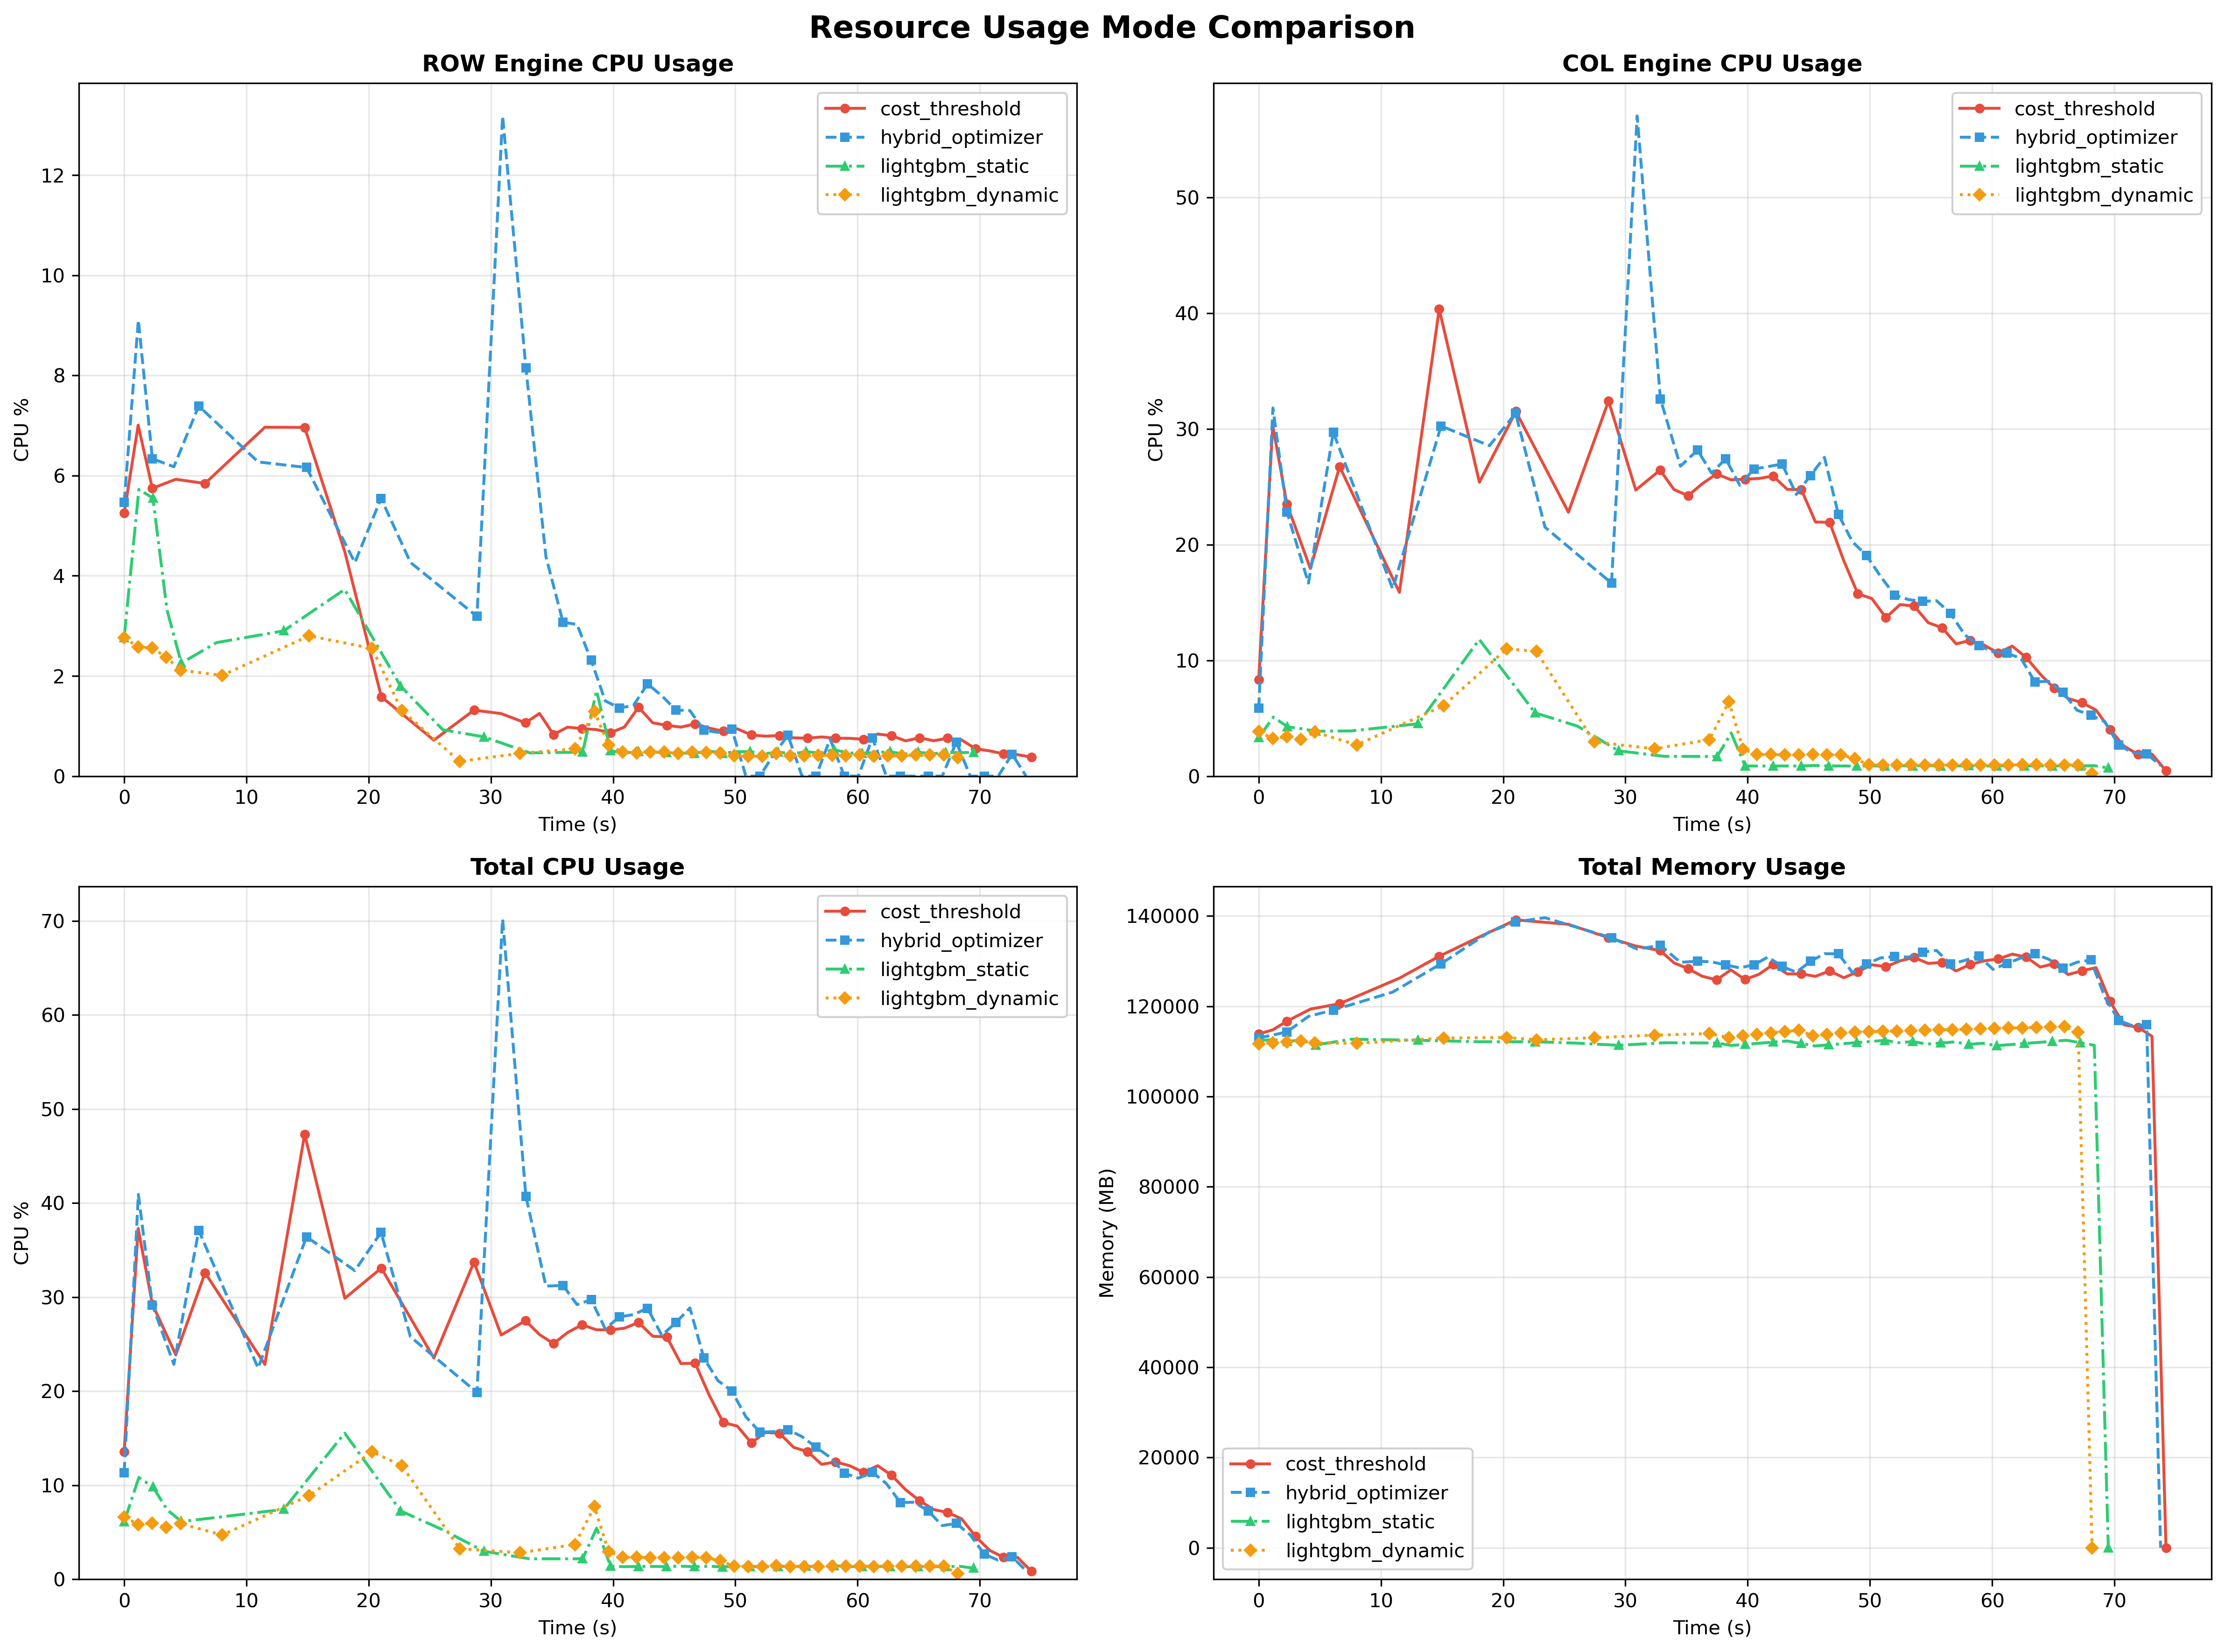
\includegraphics[width=0.8\linewidth]{figures/resource_comparison.png}
    \caption{Resource utilization profiles during 800-query concurrent execution across four dispatch strategies. Learned methods achieve stable resource consumption after initial warm-up.}
    \label{fig:resource-comparison}
\end{figure*}

\vspace{-0.5em}
\paragraph{Resource Efficiency and Stability.}
Figure~\ref{fig:resource-comparison} reveals striking differences in resource utilization during 800 concurrent query execution. Traditional strategies exhibit severe inefficiency with volatile CPU patterns—the hybrid optimizer peaks at 36\% total CPU utilization with the column engine alone consuming 29\%, while learned methods stabilize at 2-3\% after a 40-second warm-up period, achieving a 12× reduction. The column engine shows the most dramatic improvement, dropping from sustained 10-20\% usage in traditional methods to under 2\% with ML-based routing. Memory consumption further validates our approach: traditional strategies grow from 115GB to over 130GB with high volatility, while LightGBM variants maintain stable footprints around 111GB. This rapid convergence to efficient resource utilization demonstrates that intelligent query dispatch prevents engine thrashing and enables predictable performance characteristics essential for production deployments.



\subsection{Concurrent Execution on Standard Benchmarks}

We evaluate \dispatcher on industry-standard benchmarks under concurrent execution of their official template queries. Table~\ref{tab:benchmark_results} compares dispatch strategies across TPC-DS, TPC-H, and ClickBench workloads.

\begin{table}[t]
\centering
\caption{Performance on Standard Benchmarks}
\label{tab:benchmark_results}
% \vspace{-0.1in}
\resizebox{\columnwidth}{!}{%
\begin{tabular}{@{}llcc@{}}
\toprule
\textbf{Benchmark} & \textbf{Strategy} & \textbf{Makespan (s)} & \textbf{Avg Latency (s)} \\
\midrule
\multirow{4}{*}{TPC-DS} 
& Cost Threshold    & 171.84 & 104.98 \\
& Hybrid Optimizer  & 171.84 & 105.31 \\
& LightGBM Static   & 172.18 & 103.90 \\
& LightGBM Dynamic  & \textbf{171.27} & \textbf{100.50} \\
\midrule
\multirow{4}{*}{TPC-H} 
& Cost Threshold    & 145.95 & 105.63 \\
& Hybrid Optimizer  & 145.90& 106.18 \\
    & LightGBM Static   & \textbf{145.73} & 75.18  \\
& LightGBM Dynamic  & 145.76 & \textbf{74.87} \\
\midrule
\multirow{4}{*}{ClickBench} 
& Cost Threshold    & 407.77 & 48.47  \\
& Hybrid Optimizer  & 384.27 & 43.70  \\
& LightGBM Static   & 374.88 & 42.99  \\
& LightGBM Dynamic  & \textbf{373.95} & \textbf{42.78} \\
\bottomrule
\end{tabular}%
}
\vspace{-0.15in}
\end{table}

Learning-based approaches outperform traditional methods on all benchmarks. Dynamic dispatch achieves the best results: 4.3\% latency reduction on TPC-DS, 29.1\% on TPC-H, and 11.7\% on ClickBench compared to cost threshold. The performance gap between static and dynamic variants is 3.2\% on TPC-DS (3.2\%).  ClickBench shows the largest makespan improvement (8.3\%), demonstrating effectiveness on real-world workloads. These results validate that \dispatcher's adaptive approach successfully handles diverse query patterns while maintaining stable performance across different benchmark characteristics.


\begin{table}[h]
  \centering
  \small
  \setlength{\tabcolsep}{4pt}
  \caption{Hybench Benchmark Results for Different Dispatch Strategies. }
  \vspace{-0.5em}
  \label{tab:hybench}
  \resizebox{\linewidth}{!}{%
  \begin{tabular}{lccccc}
    \toprule
    \textbf{Method} & \textbf{AP-QPS} $\uparrow$ & \textbf{TP-TPS} $\uparrow$ & \textbf{XP-QPS} $\uparrow$ & \textbf{XP-TPS} $\uparrow$ & \textbf{HTAP-Score} $\uparrow$ \\
    \midrule
    Cost Threshold   & \textbf{0.21} & 29.78 & \textbf{0.68} & 0.47 & 1.93 \\
    Hybrid Optimizer & 0.20 & 20.25 & 0.62 & 0.65 & 1.73 \\
    LightGBM Static  & \textbf{0.21} & 32.77 & 0.48 & 0.68 & 2.00 \\
    LightGBM Dynamic & \textbf{0.21} & \textbf{33.97} & 0.52 & \textbf{0.78} & \textbf{2.10} \\
    \bottomrule
  \end{tabular}
  }
  \footnotesize{Note: QPS/TPS denote throughput for AP/TP workloads, XP-QPS/XP-TPS denote HTAP workload performance, and the HTAP-Score is the geometric mean across components.}
  \vspace{-1em}
\end{table}


Table~\ref{tab:hybench} compares four dispatch strategies on HTAP benchmark \texttt{hybench}~\cite{zhang2024hybench}. 
Our LightGBM-based methods (\texttt{LightGBM Static} and \texttt{LightGBM Dynamic}) achieve higher overall HTAP scores than the baselines. 
Among them, \texttt{LightGBM Dynamic} delivers the best performance (2.10), with strong gains in both transactional and mixed workloads.


\subsection{RL Learning Process}

Figure~\ref{fig:rl_learning} demonstrates the online learning behavior of our LinTS-Delta bandit. We can see the bandit is learning the residual between actual latency and estimated latency and updating adaptively, especially at the beginning and during the 1500 and 2200 queries.

\begin{figure}[h]
\centering
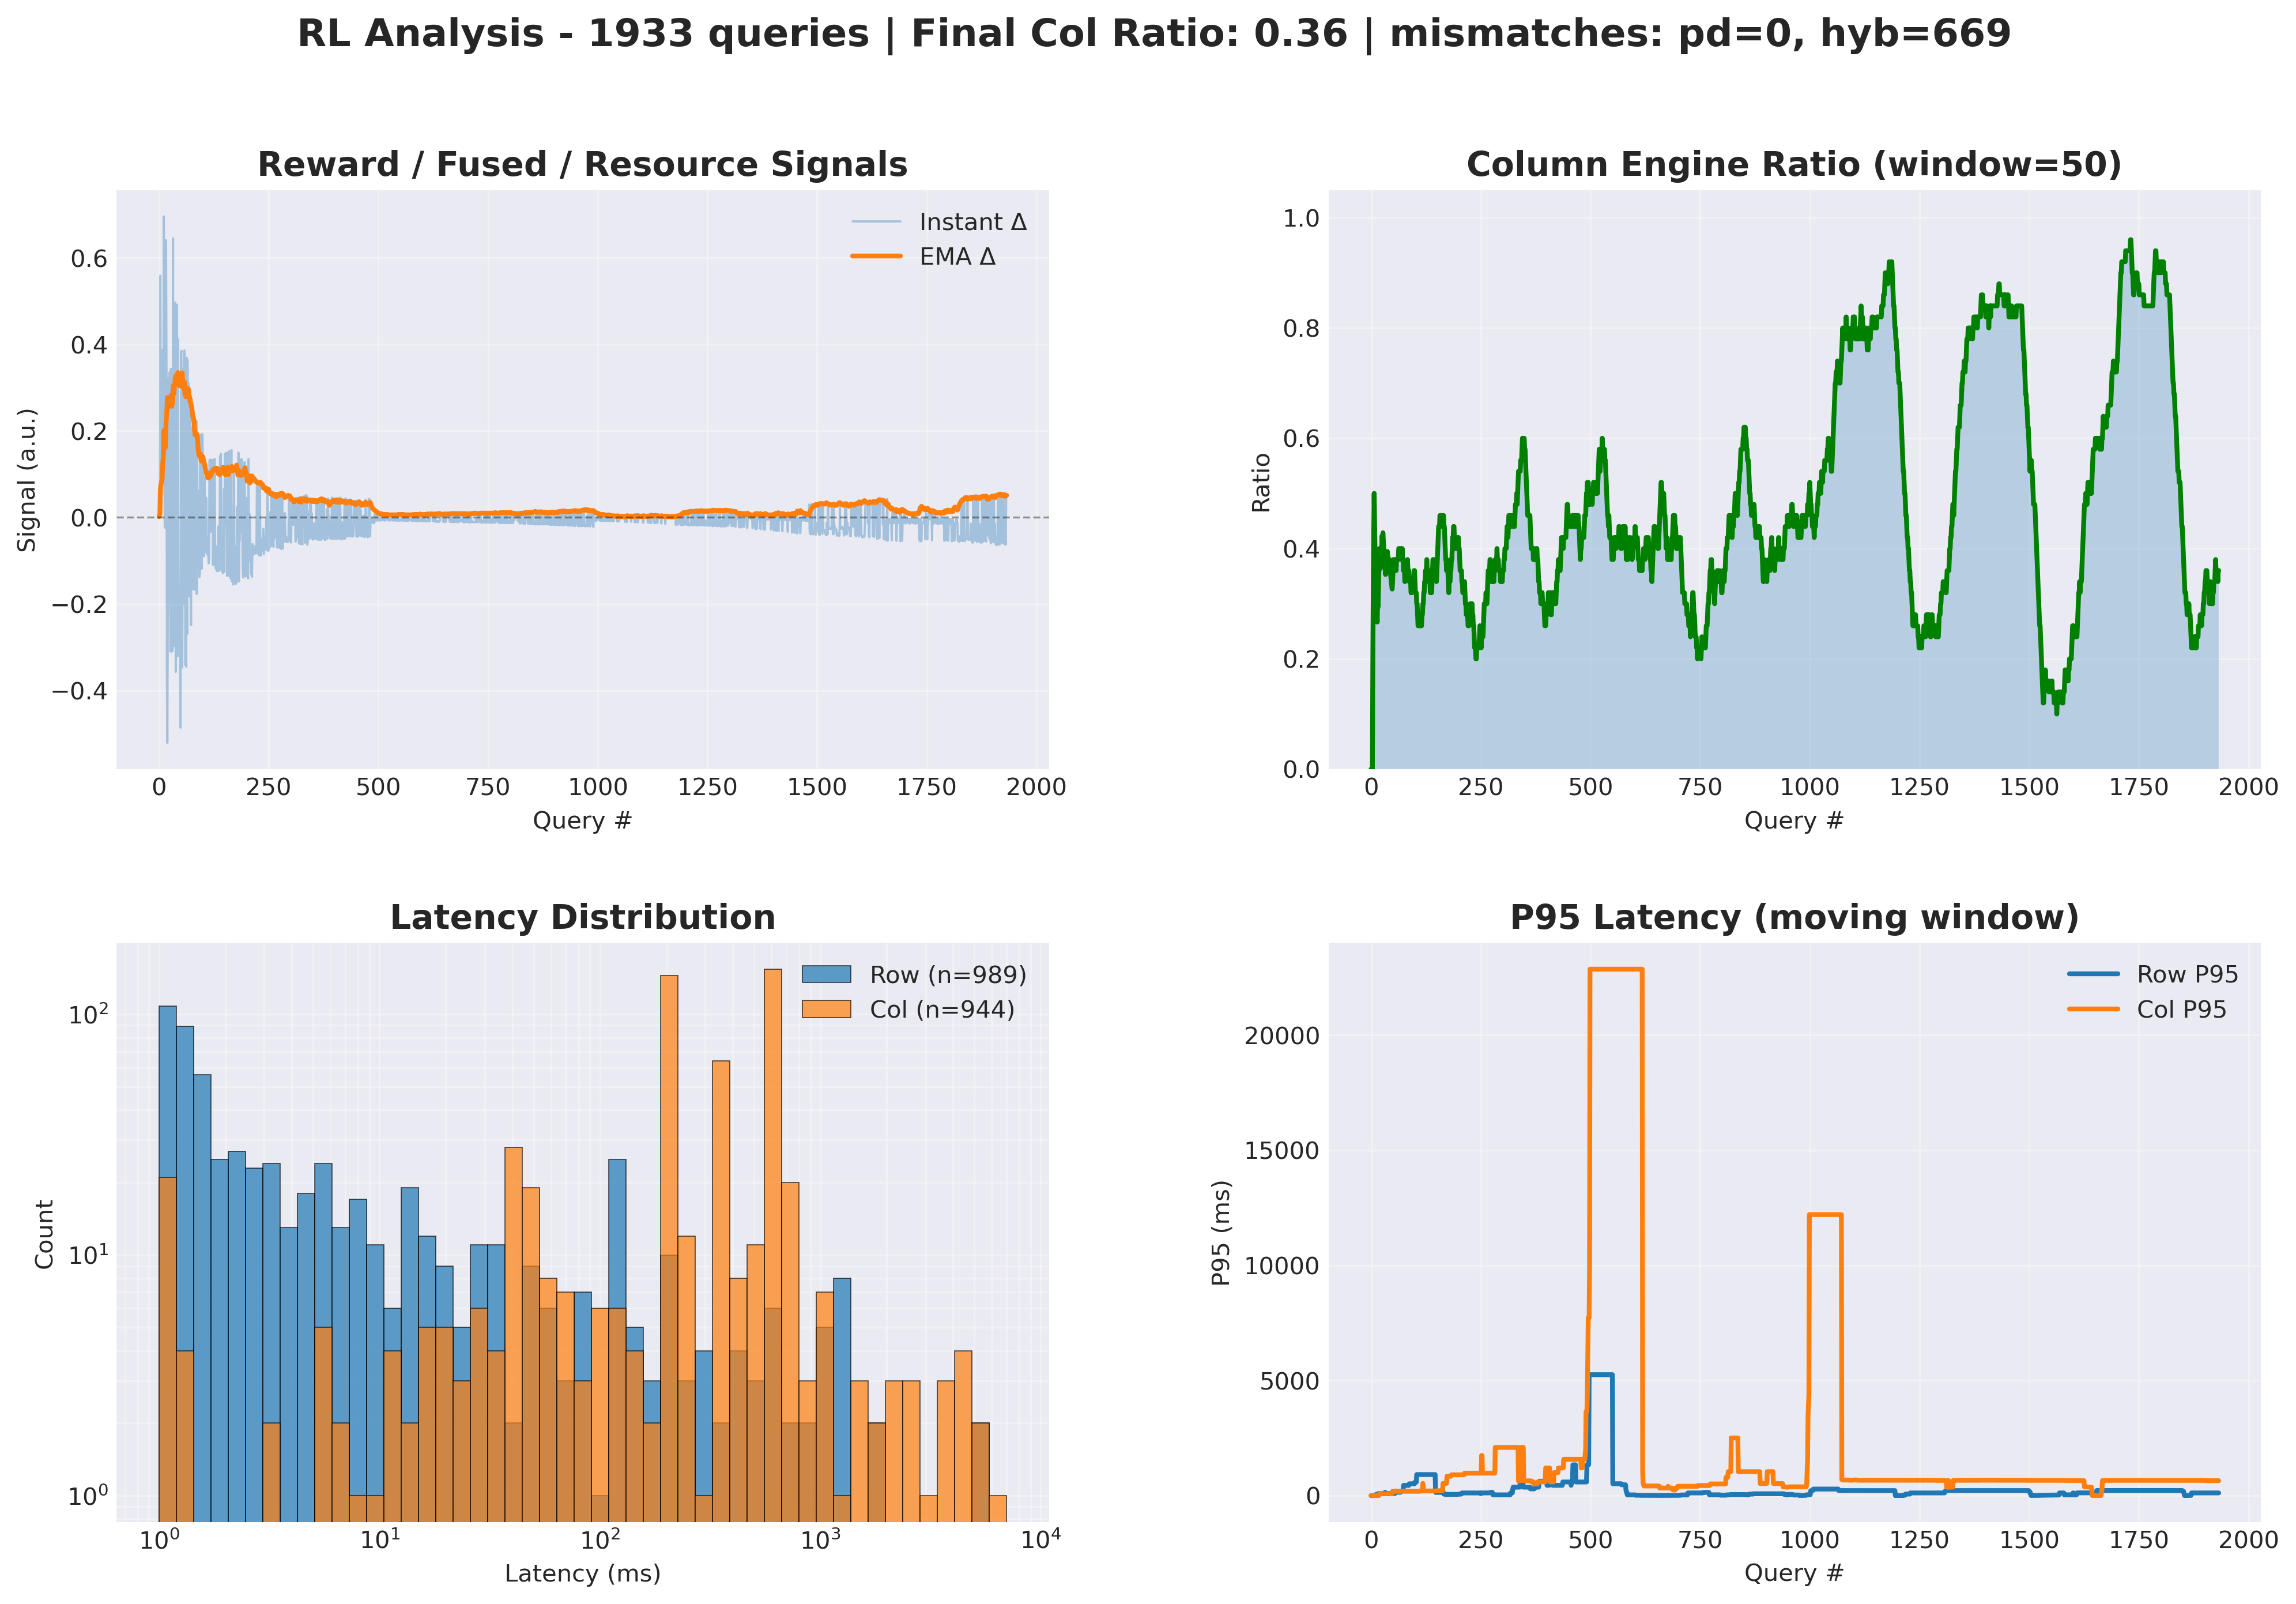
\includegraphics[width=\columnwidth]{figures/rl_analysis.png}
\caption{RL learning process}
\label{fig:rl_learning}
\vspace{-1.5em}
\end{figure}

% ============================================================
\section{Discussion}\label{sec:discussion}
% ============================================================

We analyze \dispatcher's design decisions, examine the factors driving its performance gains, and discuss limitations and future directions.

\vspace{1em}
%--------------------------------------------------------------------
\noindent
\textbf{Offline-Online Synergy.}
\dispatcher's two-phase architecture reflects a fundamental tradeoff in learned database systems: the need for both predictive accuracy and runtime adaptability.

\paragraph{Offline Learning.} The offline phase distills 142 raw features into 32 SHAP-selected signals and trains a 10MB LightGBM ensemble using regret-weighted boosting. This phase captures stable query-to-engine mappings from historical workloads, encoding complex decision boundaries that no fixed threshold can express. The model achieves up to 87\% of optimal performance on isolated queries, providing a strong foundation for runtime decisions.

\paragraph{Online Adaptation.} Runtime dynamics (resource contention, workload shifts, and queueing effects) necessitate online correction. Our LinTS-Delta bandit learns residual errors between predicted and actual performance, while the OCO-based resource controller maintains CPU/memory balance through Mahalanobis distance scoring. This dual adaptation mechanism reduces makespan by up to 52\% compared to static dispatch at high concurrency (Table~\ref{tab:routing_perf}), demonstrating that even accurate offline models benefit from online refinement.

The key insight is that offline and online components address complementary aspects: the former captures query-intrinsic properties (selectivity, join patterns), while the latter handles system-extrinsic factors (load, resource availability). This separation of concerns enables sub-millisecond decisions while maintaining theoretical guarantees on both regret and resource deviation.

%--------------------------------------------------------------------
\noindent
\textbf{Limitations and Future Directions.}
We summarize the limitations of our method as below and point out future research directions:
\begin{enumerate}[leftmargin=*,topsep=0pt,itemsep=3pt]
    \item \textbf{Plan-Level Granularity.} \dispatcher currently makes binary engine choices per query. Fine-grained operator-level dispatch could further improve performance, particularly for queries with mixed OLTP/OLAP characteristics. In the future, we plan to train machine learning model to dispatch each operator to row engine or column engine to achieve better optimization.
    \item \textbf{Model Maintenance.} While our system includes mechanisms for online adaptation, long-term model drift remains a challenge. We plan to address this through two complementary approaches:
        \begin{enumerate}[leftmargin=*]
        \item \emph{Periodic retraining}: A background process monitors prediction accuracy and triggers retraining when validation regret exceeds thresholds.
        \item \emph{Incremental learning}: During low-utilization periods, the system selectively re-executes queries on both engines to gather fresh labels, updating the model through mini-batch gradient boosting without service interruption.
        \end{enumerate}
    \item \textbf{Generalization across Systems.} \dispatcher's core principles — feature engineering, regret-weighted training, and bandit-based learning—directly apply to other dual-engine HTAP systems. The approach can be readily transferred to TiDB, MySQL HeatWave, and Postgres paired with DuckDB. Only the feature extraction layer requires system-specific adaptation, while the learning pipeline remains unchanged.
    \item \textbf{Interpretability.} Future work could integrate learned decision rules with natural language generation to produce human-readable explanations for dispatch decisions (e.g., ``Dispatched to column engine due to high join fanout (100×) on \texttt{lineitem} table with aggregation operations'').
\end{enumerate}


% ============================================================
\vspace{-1em}
\section{Related Work}\label{sec:related}
% ============================================================
%proteus. metis.  Adaptive HTAP through Elastic Resource Scheduling
We list research on HTAP architectures, query dispatch techniques, and ML-based database optimization approaches.

%--------------------------------------------------------------------
\noindent\textbf{HTAP Architectures.}
HTAP systems~\cite{zhang2024htap,song2023rethink} can be classified into:
(i) Single-Engine Systems. 
        These maintain both row and column formats within one engine.
        SAP HANA~\cite{farber2012sap_data_eng_bull} pioneered unified storage with per-operator format selection.
        Oracle Database In-Memory~\cite{lahiri2015oracle} and SQL Server Columnstore~\cite{larson2015real,dziedzic2018columnstore} 
        add columnar capabilities to row engines.
        HyPer~\cite{kemper2011hyper} uses fork-based snapshots for isolation.
        StarRocks~\cite{starrocks2025} is a modern MPP analytical database that combines a vectorized execution engine, columnar storage, and real-time ingestion to provide high-performance HTAP capabilities.
(ii) Dual-Engine Systems.
        They separate OLTP and OLAP engines with data synchronization.
        TiDB + TiFlash~\cite{huang2020tidb} uses Raft-based replication,
        ByteHTAP~\cite{chen2022bytehtap} achieves sub-second freshness,
        and PolarDB~\cite{wang2023polardb} introduces row-column fusion operators.
        SingleStore~\cite{prout2022cloud} and Snowflake Unistore~\cite{sun2023unistore} follow similar patterns.


\noindent\textbf{Query Dispatch Strategies.}
Query dispatch varies along two dimensions: granularity and methodology. Table~\ref{tab:design-space} summarizes dispatch granularities.
Static-layout engines like IBM DB2 BLU~\cite{raman2013db2} eliminate runtime decisions entirely. Plan-level dispatch, exemplified by MySQL HeatWave~\cite{oracle2025heatwave}, dispatches entire queries to a single engine, balancing flexibility with implementation simplicity. Operator-level systems—including SQL Server~\cite{larson2015real}, Oracle In-Memory~\cite{lahiri2015oracle}, SAP HANA~\cite{krueger2010optimizing}, TiDB~\cite{huang2020tidb}, and PolarDB~\cite{wang2023polardb} — enable fine-grained per-operator engine selection, maximizing performance potential at the cost of increased optimization complexity.

\begin{table}[t]
  \caption{Design space for row/column dispatch strategies.}
  \label{tab:design-space}
  %\vspace{-1em}
  \small
  \setlength{\tabcolsep}{3pt}
  \renewcommand{\arraystretch}{1.2}
  \renewcommand{\tabularxcolumn}[1]{m{#1}}  % 添加此行以垂直居中 X 列

  \begin{tabularx}{\columnwidth}{@{} 
  >{\raggedright\arraybackslash\hsize=0.9\hsize}X 
  >{\raggedright\arraybackslash\hsize=1.1\hsize}X 
  >{\raggedright\arraybackslash\hsize=1\hsize}X @{}}
    \toprule
    \textbf{Granularity} &
    \qquad \textbf{Pros} &
    \qquad \textbf{Cons}\\
    \midrule
    Static layout~\cite{raman2013db2} &
      (1) No run-time choice; (2) simple &
      (1) Cannot combine row and column strengths \\[2pt]
    Plan-level~\cite{oracle2025heatwave} &
      (1) Smaller search space; (2) No intra-query engine switches &
      (1) Cannot mix layouts when only part of a plan benefits \\[2pt]
    Operator-level~\cite{larson2015real,lahiri2015oracle,huang2020tidb,wang2023polardb,farber2012sap_acm} &
      (1) Highest potential performance; (2) Fine-grained optimisation &
      (1) Large search space; (2) More complex implementation \\
    \bottomrule
  \end{tabularx}
  \vspace{-1em}
\end{table}

Dispatch methodologies include cost-based, rule-based, and learning\hspace{0pt}-based.
Most systems employ cost models~\cite{wang2023polardb,larson2015real} or manually tuned heuristics~\cite{farber2012sap_acm}. 
Recent work explores machine learning: ByteHTAP~\cite{chen2022bytehtap} mentions that it applies tree-CNNs for plan-level dispatch decisions but does not provide experimental results. 
However, existing dispatch approaches remain static after deployment, unable to adapt to workload shifts or system dynamics.

\noindent\textbf{Learning-Based Database Optimization.}
Recent work has explored machine learning for database optimization. Neo and Bao enhance traditional cost models using gradient-boosted trees~\cite{marcus2019neo,marcus2021bao}, while Wu et al. apply graph neural networks for query memory prediction~\cite{wu2025memq}. Online learning approaches include deep RL for join ordering~\cite{krishnan2018learning} and multi-armed bandits for index selection~\cite{perera2021dba,wu2024automatic}. Resource-aware schedulers such as Auto-WLM~\cite{saxena2023auto}, LSched~\cite{sabek2022lsched}, and buffer-sensitive RL~\cite{zhang2020buffer} incorporate system constraints but do not address query-level row/column dispatch under dynamic HTAP workloads. Our work fills this gap by combining offline learning with online adaptation for dispatch decisions that balance performance and resource utilization.

\section{Conclusion}\label{sec:conclusion}
\dispatcher combines supervised learning, contextual bandits, and resource-aware control to improve query dispatch in HTAP systems. Our prototype implementation in PolarDB achieves up to 42\% latency reduction across diverse workloads, reaching 87\% of optimal performance. Under high concurrency, the system reduces latency by over 40\% while maintaining stable resource utilization, with approximately 500 $\mu$s dispatch overhead. The key finding is that integrating offline prediction with online adaptation outperforms single-model approaches. This work demonstrates the feasibility of our online adaptive query dispatcher framework in HTAP database systems.



%\begin{acks}
% This work was supported by the [...] Research Fund of [...] (Number [...]). Additional funding was provided by [...] and [...]. We also thank [...] for contributing [...].
%\end{acks}


\clearpage
\bibliographystyle{ACM-Reference-Format}
\bibliography{sample}



\end{document}
\endinput
